\documentclass[11pt,a4paper,oneside]{scrartcl}

\newcommand{\mchname}{Mat\'{u}\v{s} Chochl\'{i}k}
\newcommand{\mchmail}{chochlik@gmail.com}
\newcommand{\docname}{Static reflection (rev. 3)}
\newcommand{\docnum}{N4451}
\newcommand{\docdate}{2015-04-11}

\usepackage[utf8]{inputenc}
\usepackage{url}
\usepackage[colorlinks=true]{hyperref}
\usepackage{parskip}
\usepackage[titletoc]{appendix}

\usepackage{listings}
\usepackage{minted}
\lstset{basicstyle=\footnotesize\ttfamily,breaklines=true}

\usepackage{fancyhdr}
\setlength{\headheight}{14pt}
\pagestyle{fancyplain}
\lhead{\fancyplain{}{\docnum - \docname}}
\rhead{}
\rfoot{\fancyplain{}{\thepage}}
\cfoot{}

\usepackage[pdftex]{graphicx}
\DeclareGraphicsExtensions{.pdf,.png,.jpg,.mps,.eps}
\graphicspath{{images/}}

\usepackage{tikz}
\usetikzlibrary{arrows,positioning}
\tikzstyle{concept}=[
	rectangle,	
	very thick,
	draw=red!80!black!80,
	top color=white,
	bottom color=red!20,
	node distance=0.5em and 1.5em
]
\tikzstyle{inheritance}=[
	->,
	shorten >=1pt,
	>=open triangle 90,
	very thick
]
   

\setcounter{tocdepth}{3} 

\title{\docname}

\author{\mchname (\mchmail)}

\newcommand{\concept}[1]{\hyperref[concept-#1]{\em{#1}}}
\newcommand{\meta}[1]{\concept{Meta#1}}

\begin{document}

\begin{tabular}{r l}
Document number: & \docnum\\
Date: & \docdate\\
Project: & Programming Language C++, SG7, Reflection\\
Reply-to: & \mchname (\href{mailto:\mchmail}{\mchmail})\\
\end{tabular}

\begin{center}
\vskip 2em
{\Huge \docname}
\vskip 1em
{\emph \mchname}
\vskip 2em
\end{center}

\paragraph{Abstract}

This paper is the follow-up to N3996 and N4111 an it is the third revision
of the proposal to add support for static reflection to the C++ standard.
During the presentation of N4111 concerns were expressed about the level-of-detail and scope
of the presented proposal and possible dangers of giving non-expert language users
a {\em too powerful} tool to use and the dangers of implementing it all at once.
This paper aims to address these issues.
Furthermore the accompanying paper -- N4452 describes several use cases of reflection,
which were called for during the presentation of N4111.

\tableofcontents

\section{Introduction}

Reflection and reflective programming can be used
for a wide range of tasks such as implementation of serialization-like operations,
remote procedure calls, scripting, automated GUI-generation,
implementation of several software design patterns, etc.
C++ as one of the most prevalent programming languages 
lacks a standardized reflection facility.

In this paper we propose the addition of native support for
compile-time reflection to C++ and a library built
on top of the metadata provided by the compiler.

The basic static metadata provided by compile-time reflection
should be as complete as possible to be applicable in a wide
range of scenarios and allow to implement custom higher-level
static and dynamic reflection libraries and reflection-based
utilities.

The term \emph{reflection} refers to the ability of a computer program
to observe and possibly alter its own structure and/or its behavior.
This includes building new or altering the existing data structures,
doing changes to algorithms or changing the way the program code
is interpreted. Reflective programming is a particular kind
of \emph{metaprogramming}.

The advantage of using reflection is in the fact that everything
is implemented in a single programming language, and the human-written
code can be closely tied with the customizable reflection-based
code which is automatically generated by compiler metaprograms,
based on the metadata provided by reflection.

The solution proposed in this paper is based on the
\href{http://kifri.fri.uniza.sk/~chochlik/mirror-lib/html/}{\em Mirror}
reflection utilities~\cite{mirror-doc-cpp11} and on several years
of user experience with reflection-based metaprogramming.

\section{Currently proposed metaobject concepts}
\label{section-current-Concepts}

We propose that the basic metadata describing a program written
in C++ should be made available through a set of {\em anonymous} types
defined by the compiler and through related functions and template classes.
At the moment these types should describe only the following program
constructs: namespaces\footnote{in a very limited form}, types, typedefs,
classes and their data members.

In the future, the set of metaobjects should be extended to reflect also
class inheritance, free functions, class member functions, templates,
template parameters, enumerated values, specifiers, etc.
See appendix~\ref{section-all-Concepts} for more details.

The compiler should generate metadata for the program constructs defined
in the currently processed translation unit. Members of ordered sets (ranges) of metaobjects,
like scope members, parameters of a function, and so on, should be listed
in the order of appearance in the processed source code.

Since we want the metadata to be available at compile-time,
different base-level constructs should be reflected by
{\em statically different} metaobjects and thus by {\em different} types.
For example a metaobject reflecting the global scope namespace should
be a different {\em type} than a metaobject reflecting the \verb@std@
namespace\footnote{this means that they should be distinguishable for
example by the \texttt{std::is\_same} type trait},
a metaobject reflecting the \verb@int@ type should
have a different type then a metaobject reflecting the \verb@double@
type, etc.

In a manner of speaking these metaobjects should become
"instances" of the meta-level concepts\footnote{conceptual interfaces which
describe the requirements of types modelling them, but
should not exist as concrete types}, but rather only at the
"specification-level" similar for example to the iterator concepts.

This section describes a set of metaobject concepts,
their interfaces\footnote{the requirements that the various metaobjects
need to satisfy in order to be considered models of the individual
concepts},
tag types for metaobject classification and
functions (or operators) providing access to the metaobjects.

Unless stated otherwise, all named templates proposed and described below should
go into the \verb@std@ namespace. Alternatively, if any of the definitions
proposed here would clash with existing members (or new members proposed elsewhere)
of the \verb@std@ namespace, then they can be nested in a namespace like
\verb@std::meta@ or \verb@std::mirror@.

Also note, that in the sections below, the examples use names for concrete
metaobjects, like \verb@__meta_std_string@, etc. This convention
is {\em NOT} part of this proposal. The actual naming of the metaobjects
should be left to the compiler implementations and for all purposes,
from the users point of view, the metaobjects should be anonymous types.

\subsection{Categorization and Traits}

In order to provide means for distinguishing between regular types
and metaobjects generated by the compiler,
the \verb@is_metaobject@ trait should be added to the \verb@std@ namespace\footnote{
even if a nested namespace like \texttt{std::meta} is used for everything else}
and should inherit from \verb@true_type@ for metaobjects\footnote{types generated
by the compiler providing metadata} and from \verb@false_type@
for non-metaobjects\footnote{native or user defined types}:

\begin{minted}{cpp}
template <typename T>
struct is_metaobject
 : false_type
{ };
\end{minted}

\subsubsection{Metaobject category tags}
\label{metaobject-category-tags}

To distiguish between various metaobject kinds\footnote{metaobjects satisfying different concepts
as described below} a set of tag \verb@struct@s indicating the kind of the metaobject
should be added:

\begin{minted}{cpp}
struct specifier_tag
{
	typedef specifier_tag type;
};

struct namespace_tag
{
	typedef namespace_tag type;
};

struct global_scope_tag
{
	typedef global_scope_tag type;
};

struct type_tag
{
	typedef type_tag type;
};

struct typedef_tag
{
	typedef typedef_tag type;
}; 

struct class_tag
{
	typedef class_tag type;
};

struct function_tag
{
	typedef function_tag type;
};

struct constructor_tag
{
	typedef constructor_tag type;
};

struct operator_tag
{
	typedef operator_tag type;
};

struct overloaded_function_tag
{
	typedef overloaded_function_tag type;
};

struct enum_tag
{
	typedef enum_tag type;
};

struct enum_class_tag
{
	typedef enum_class_tag type;
};

struct inheritance_tag
{
	typedef inheritance_tag type;
};

struct constant_tag
{
	typedef constant_tag type;
};

struct variable_tag
{
	typedef variable_tag type;
};

struct parameter_tag
{
	typedef parameter_tag type;
};
\end{minted}

These tags are referred-to as \verb@MetaobjectCategory@ below:

\subsubsection{Specifier category tags}
\label{specifier-category-tags}

Similar to the \hyperref[metaobject-category-tags]{metaobject tag} types,
a set of tag types for individual C++ specifier keywords should be defined:

\begin{minted}{cpp}
// indicates no specifier
struct none_tag
{
	typedef none_tag type;
};

struct extern_tag
{
	typedef extern_tag type;
};

struct static_tag
{
	typedef static_tag type;
};

struct mutable_tag
{
	typedef mutable_tag type;
};

struct register_tag
{
	typedef register_tag type;
};

struct thread_local_tag
{
	typedef thread_local_tag type;
};

struct const_tag
{
	typedef const_tag type;
};

struct virtual_tag
{
	typedef virtual_tag type;
};

struct private_tag
{
	typedef private_tag type;
};

struct protected_tag
{
	typedef protected_tag type;
};

struct public_tag
{
	typedef public_tag type;
};

struct class_tag
{
	typedef class_tag type;
};

struct struct_tag
{
	typedef struct_tag type;
};

struct union_tag
{
	typedef union_tag type;
};

struct enum_tag
{
	typedef enum_tag type;
};

struct enum_class_tag
{
	typedef enum_class_tag type;
};

struct constexpr_tag
{
	typedef constexpr_tag type;
};

\end{minted}

These tags are collectively referred-to as \verb@SpecifierCategory@ below.

\subsection{StringConstant}
\label{concept-StringConstant}

A \concept{StringConstant} is a class conforming to the following:

\begin{minted}{cpp}
struct StringConstant
{
	typedef StringConstant type;

	// null terminated char array with size (string length+1)
	// known to sizeof at compile-time
        static constexpr const char value[Length+1] = {..., '\0'};

	// implicit compile-time conversion to null terminated
	// c-string
        constexpr operator const char* (void) const
        {
                return value;
        }
};

constexpr const char StringConstant::value[Length+1];
\end{minted}

Concrete models of \concept{StringConstant} are used to return compile-time string values.
For example the \verb@_str_void@ type defined below, conforms to the \concept{StringConstant}
concept:

\begin{minted}{cpp}
template <char ... C>
struct string_constant
{
	typedef string_constant type;

	static constexpr const char value[sizeof...(C)+1] = {C...,'\0'};

	constexpr operator const char* (void) const
	{
		return value;
	}
};

template <char ... C>
constexpr const char string_constant::value[sizeof...(C)+1];

//...

typedef string_constant<'v','o','i','d'> _str_void;

cout << _str_void::value << std::endl;
cout << _str_void() << std::endl;
static_assert(sizeof(_str_void::value) == 4+1, "");
\end{minted}

The strings stored in the \verb@value@ array should be UTF-8 encoded.

\textbf{Note:} the \verb@string_constant@ class as defined above is just one of the
possible implementations of \concept{StringConstant}, we do not however imply
that it must be implemented this way.

\subsection{Metaobject Sequence}
\label{concept-MetaobjectSequence}

As the name implies \concept{MetaobjectSequence}s are used to store seqences
or tuples of metaobjects.
A model of \concept{MetaobjectSequence} is a class conforming to the following:

It is a nullary metafunction returning itself:

\begin{minted}{cpp}
template <typename Metaobject>
struct MetaobjectSequence
{
	typedef MetaobjectSequence type;
};
\end{minted}

\textbf{Note:} The definition above is only a psedo-code and
the template parameter \verb@Metaobject@ indicates here the minimal
metaobject concept which all elements in the sequence must satisfy.
For example a \verb@MetaobjectSequence<MetaConstructor>@ denotes a sequence
of metaobjects that all satisfy the \meta{Constructor} concept, etc.

\subsubsection{\texttt{size}}

A template class \verb@size@ is defined as follows:

\begin{minted}{cpp}
template <typename T>
struct size;

template <>
struct size<MetaobjectSequence<Metaobject>>
 : integral_type<size_t, N>
{ };
\end{minted}

Where \verb@N@ is the number of elements in the sequence.

\subsubsection{\texttt{at}}

A template class \verb@at@, providing random access to metaobjects in a sequence
is defined (for values of \verb@I@ between \verb@0@ and \verb@N-1@ where \verb@N@
is the number of elements returned by \verb@size@) as follows:

\begin{minted}{cpp}
template <typename T, size_t I>
struct at;

template <size_t I>
struct at<MetaobjectSequence<Metaobject>, I>
 : Metaobject
{ };
\end{minted}

For example if \verb@__meta_seq_ABC@ is a metaobject sequence containing three metaobjects;
\verb@__meta_A@, \verb@__meta_B@ and \verb@__meta_C@ (in that order), then:

\begin{minted}{cpp}
template <>
struct size<__meta_seq_ABC>
 : integral_constant<size_t, 3>
{ };
\end{minted}

and 

\begin{minted}{cpp}
template <>
struct at<__meta_seq_ABC, 0>
 : __meta_A
{ };

template <>
struct at<__meta_seq_ABC, 1>
 : __meta_B
{ };

template <>
struct at<__meta_seq_ABC, 2>
 : __meta_C
{ };
\end{minted}

\textbf{Note:} The order of the metaobjects in a sequence is determined by the order
of appearance in the processed translation unit.

\subsubsection{\texttt{for\_each}}

A template function \verb@for_each@ should be defined and should
execute the specified unary function on every \meta{object} in
the sequence, in the order of appearance in the processed translation unit.

\begin{minted}{cpp}
template <typename MetaobjectSequence, typename UnaryFunc>
void for_each(UnaryFunc func)
{
	func(Metaobject1());
	func(Metaobject2());
	/* ... */
	func(MetaobjectN());
}

\end{minted}

This design requires the metaobjects to be default constructible.
If this should prove to be a problem then an \verb@identity@ wrapper could be used
instead:

\begin{minted}{cpp}
template <typename X>
struct identity
{
	typedef X type;
};

template <typename MetaobjectSequence, typename UnaryFunc>
void for_each(UnaryFunc func)
{
	func(identity<Metaobject1>());
	func(identity<Metaobject2>());
	/* ... */
	func(identity<MetaobjectN>());
}

\end{minted}

\textbf{Note:} The interface of \meta{objectSequence}, in particular \verb@size@
and \verb@at@ together with \verb@std::index_sequence@ should be enough
to implement a single generic version of \verb@for_each@.


\subsection{Metaobject}
\label{concept-Metaobject}

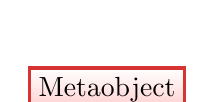
\begin{tikzpicture}
\node[concept] (Metaobject) {Metaobject};
\end{tikzpicture}

A \meta{object} is a stateless anonymous type generated by the compiler which
provides metadata reflecting a specific program feature. Each metaobject
should satisfy the following:

Every metaobject should be a nullary metafunction returning itself:

\begin{minted}{cpp}
struct Metaobject
{
	typedef Metaobject type;
};
\end{minted}

One possible way how to achieve this is to define {\em basic metaobjects}
as plain types (without any internal structure) and define a class template like:

\begin{minted}{cpp}
template <typename BasicMetaobject>
struct metaobject
{
	typedef metaobject type;
};
\end{minted}

and then, implement the actual \meta{object}s as instantiations of this template.
For example if \verb@__base_meta_int@ is a basic metaobject reflecting the \verb@int@
type then the actual metaobject \verb@__meta_int@ conforming to this concept could 
be defined as:

\begin{minted}{cpp}
typedef metaobject<__base_meta_int> __meta_int;
\end{minted}

Although, this is just one possibility not a requirement of this proposal.

\subsubsection{\texttt{is\_metaobject}}

The \verb@is_metaobject@ template should inherit from \verb@true_type@ for all \meta{object}s,
and inherit from \verb@false_type@ otherwise.

\begin{minted}{cpp}
template <typename T>
struct is_metaobject
 : false_type
{ };

template <>
struct is_metaobject<Metaobject>
 : true_type
{ };
\end{minted}

\subsubsection{\texttt{metaobject\_category}}

A template class \verb@metaobject_category@ should be defined in the \verb@std@ namespace
(even if everything else is defined inside of a nested namespace like \verb@std::meta@)
and should inherit from
one of the \hyperref[metaobject-category-tags]{metaobject category tags}, depending on
the actual kind of the metaobject.

\begin{minted}{cpp}
template <typename T>
struct metaobject_category;

template <>
struct metaobject_category<Metaobject>
 : MetaobjectCategory
{ };
\end{minted}

For example if the \verb@__meta_std@ metaobject reflects the \verb@std@ namespace,
then the specialization of \verb@metaobject_category@ should be:

\begin{minted}{cpp}
template <>
struct metaobject_category<__meta_std>
 : namespace_tag
{ };
\end{minted}

\subsubsection{Comparison}

A template class \verb@equal@ should be defined and should inherit from \verb@true_type@
if a \hyperref[section-Library]{metaobject expression} \verb@Expr1@ {\em evaluates} into
the same metaobject as the metaobject expression \verb@Expr2@ (i.e. into metaobjects
that both reflect the same base-level construct). Otherwise it should inherit from
\verb@false_type@:

\begin{minted}{cpp}
template <typename Expr1, typename Expr2>
struct equal
 : BooleanConstant
{ };
\end{minted}

\subsubsection{Traits}

The following template classes indicating various properties of a \meta{object}
should be defined and should by default inherit from \verb@false_type@ unless stated
otherwise below:

\verb@has_name@ -- indicates that a \meta{object} is a \meta{Named}:
\begin{minted}{cpp}
template <typename T>
struct has_name
 : false_type
{ };
\end{minted}

\verb@has_scope@ -- indicates that a \meta{object} is a \meta{Scoped}:
\begin{minted}{cpp}
template <typename T>
struct has_scope
 : false_type
{ };
\end{minted}

\verb@is_scope@ -- indicates that a \meta{object} is a \meta{Scope}:
\begin{minted}{cpp}
template <typename T>
struct is_scope
 : false_type
{ };
\end{minted}

\verb@has_name@ -- indicates that a \meta{object} is a \meta{Positional}:
\begin{minted}{cpp}
template <typename T>
struct has_position
 : false_type
{ };
\end{minted}

\verb@is_class_member@ -- indicates that a \meta{object} is a \meta{ClassMember}:
\begin{minted}{cpp}
template <typename T>
struct is_class_member
 : false_type
{ };
\end{minted}

\verb@has_template@ -- indicates that a \meta{object} is a \meta{Instantiation}:
\begin{minted}{cpp}
template <typename T>
struct has_template
 : false_type
{ };
\end{minted}

\verb@is_template@ -- indicates that a \meta{object} is a \meta{Template}
or \meta{TemplateParameter}:
\begin{minted}{cpp}
template <typename T>
struct is_template
 : false_type
{ };
\end{minted}

\subsubsection{\texttt{source\_file}}

A template class \verb@source_file@ should be defined and should return the
path to the source file where the base-level construct reflected by a
metaobject is defined (similar to what the preprocessor \verb@__FILE__@ macro
expands to).

\begin{minted}{cpp}
template <typename T>
struct source_file;

template <>
struct source_file<MetaObject>
 : StringConstant
{ };
\end{minted}

For base-level constructs like namespaces which don't have a single specific
declaration, an empty string should be returned.

\subsubsection{\texttt{source\_line}}

A template class \verb@source_line@ should be defined and should return the (positive)
line number in the source file where the base-level construct reflected by a
metaobject is defined (similar to what the preprocessor \verb@__LINE__@ symbol
expands to).

\begin{minted}{cpp}
template <typename T>
struct source_line;

template <>
struct source_line<MetaObject>
 : integral_constant<unsigned, Line>
{ };
\end{minted}

For base-level constructs like namespaces which don't have a single specific
declaration, line number zero should be returned.


\subsection{MetaSpecifier}
\label{concept-MetaSpecifier}

\meta{Specifier} is a \meta{object} reflecting a C++ specifier. There also should be a "none"
\meta{Specifier} reflecting a missing specifier. For example the \verb@const@ specifier
on member functions can be either specified or not. In the latter case this "none" \meta{Specifier}
should be "returned".


In addition to the requirements inherited from \meta{object}, types conforming to this concept
must satisfy the following:

The \verb@category@ template should return \verb@specifier_tag@ for all \meta{Specifier}s.

\begin{minted}{cpp}
template <>
struct category<MetaSpecifier>
 : specifier_tag
{ };
\end{minted}

\subsubsection{\texttt{category}}

A template struct \verb@category@ should be defined and should inherit from one of the
\hyperref[specifier-category-tags]{specifier category tags}, depending on
the actual reflected specifier.

\begin{minted}{cpp}
template <typename T>
struct category;

template <>
struct category<MetaSpecifier>
 : SpecifierCategory
{ };
\end{minted}

For example if the \verb@__meta_static@ metaobject reflects the \verb@static@
C++ specifier, then the specialization of \verb@category@
should be:

\begin{minted}{cpp}
template <>
struct category<__meta_static>
 : static_tag
{ };
\end{minted}

If \verb@__meta_nospec@ is the \meta{Specifier} reflecting the "none" (missing) specifier,
then the specialization of \verb@category@ should be:

\begin{minted}{cpp}
template <>
struct category<__meta_nospec>
 : none_tag
{ };
\end{minted}


\subsubsection{\texttt{keyword}}

A template struct \verb@keyword@ should be defined and should return
the keyword matching the reflected specifier as a
\concept{StringConstant}.

\begin{minted}{cpp}
template <typename T>
struct keyword;

template <>
struct keyword<MetaSpecifier>
 : StringConstant
{ };
\end{minted}

For example if the \verb@__meta_thread_local@ metaobject reflects the \verb@thread local@
specifier, then the matching specialization of \verb@keyword@ could be following:

\begin{minted}{cpp}
template <>
struct keyword<__meta_thread_local>
 : string_constant<'t','h','r','e','a','d',' ','l','o','c','a','l'>
{ };
\end{minted}

If \verb@__meta_nospec@ is the \meta{Specifier} reflecting the "none" (missing) specifier,
then the specialization of \verb@keyword@ should return an empty string constant.
For example:

\begin{minted}{cpp}
template <>
struct keyword<__meta_nospec>
 : string_constant<>
{ };
\end{minted}

The \verb@string_constant<'t','h','r','e','a','d',' ','l','o','c','a','l'>@
and the \verb@string_constant<>@ classes should be models of \concept{StringConstant}
as described above.


\subsection{MetaNamed}
\label{concept-MetaNamed}

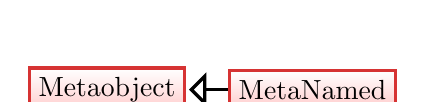
\begin{tikzpicture}
\node[concept] (Metaobject) {Metaobject};
\node[concept] (MetaNamed) [right=of Metaobject] {MetaNamed}
	edge[inheritance] (Metaobject);
\end{tikzpicture}

\meta{Named} is a \meta{object} reflecting program constructs, which have a name
(are identified by an identifier) like namespaces, types, functions, variables, parameters, etc.

In addition to the requirements inherited from \meta{object}, the following requirements must
be satisfied:

The \verb@has_name@ template class specialization for a \meta{Named} should
inherit from \verb@true_type@:

\begin{minted}{cpp}
template <>
struct has_name<MetaNamed>
 : true_type
{ };
\end{minted}

\subsubsection{\texttt{base\_name}}

A template class \verb@base_name@ should be defined an should return the base name
of the reflected construct, without the nested name specifier nor any qualifications
or other decorations, as a
\concept{StringConstant}:

\begin{minted}{cpp}
template <typename T>
struct base_name;

template <>
struct base_name<MetaNamed>
 : StringConstant
{ };
\end{minted}

For example, if \verb@__meta_std_size_t@ reflects the \verb@std::size_t@ type,
then the matching specialization of \verb@base_name@ could be implemented in the following
way:

\begin{minted}{cpp}
template <>
struct base_name<__meta_std_size_t>
 : string_constant<'s','i','z','e','_','t'>
{ };
\end{minted}

where the \verb@string_constant<'s','i','z','e','_','t'>@ class is a model
of \concept{StringConstant} as described above.

For namespace \verb@std@ the value should be \verb@"std"@, for namespace
\verb@foo::bar::baz@ it should be \verb@"baz"@, for the global scope the
value should be an empty string.

For \verb@unsigned long int * const *@ it should be \verb@"unsigned long int"@.

For \verb@std::vector<int>::iterator@ it should be \verb@"iterator"@. For derived,
qualified types like \verb@volatile std::vector<const foo::bar::fubar*> * const *@
it should be \verb@"vector"@, etc.

\subsubsection{\texttt{full\_name}}

A template class \verb@full_name@ should be defined and should return the fully
qualified name of the reflected construct, including the nested name specifier
and all qualifiers.

For namespace \verb@std@ the value 
should be \verb@"std"@, for namespace \verb@foo::bar::baz@ the value should
be \verb@"foo::bar::baz"@, for the global scope the value should be an empty
\concept{StringConstant}.
For \verb@std::vector<int>::iterator@ it should be \verb@"std::vector<int>::iterator"@.
For derived qualified types like
\verb@volatile std::vector<const foo::bar::fubar*> * const *@ it should be defined as
\verb@"volatile std::vector<const foo::bar::fubar*> * const *"@, etc.

\begin{minted}{cpp}
template <typename T>
struct full_name;

template <>
struct full_name<MetaNamedScoped>
 : StringConstant
{ };
\end{minted}

\subsubsection{\texttt{named\_typedef}}

A template class \verb@named_typedef@ should be defined:

\begin{minted}{cpp}
template <typename X, typename T>
struct named_typedef;

template <typename X>
struct named_typedef<X, MetaNamedScoped>
{
	typedef X <NAME>;
};
\end{minted}

The \verb@<NAME>@ expression above should be replaced in the actual specialization generated by the compiler
by the name of the reflected named object. If the generated identifier would clash with a C++
reserved keyword, then a single trailing underscore should be appended to the identifier.
If the generated identifier consists of multiple whitespace separated words then the whitespaces
should be replaced by a single underscore.

For example if a type \verb@__meta_std_thread@
reflects the \verb@std::thread@ class, then the specialization of \verb@named_typedef@
for this metaobject should be following:

\begin{minted}{cpp}
template <typename X>
struct named_typedef<X, __meta_std_thread>
{
	typedef X thread;
};
\end{minted}

if a type \verb@__meta_std@ reflects the \verb@std@ namespace, then the specialization of \verb@named_typedef@
should be:

\begin{minted}{cpp}
template <typename X>
struct named_typedef<X, __meta_std>
{
	typedef X std;
};
\end{minted}

if a type \verb@__meta_@ reflects the global scope (or another anonymous base-level object),
then the specialization of \verb@named_typedef@ should be:

\begin{minted}{cpp}
template <typename X>
struct named_typedef<X, __meta_>
{
	typedef X _;
};
\end{minted}

If the types \verb@__meta_int@ and \verb@__meta_unsigned_long_long_int@ reflect the \verb@int@ and
the \verb@unsigned long long int@ type
respectively, then the matching instantiations of \verb@named_typedef@ should be:

\begin{minted}{cpp}
template <typename X>
struct named_typedef<X, __meta_int>
{
	// note the trailing underscore
	typedef X int_;
};

template <typename X>
struct named_typedef<X, __meta_long_long_unsigned_int>
{
	// note underscores replacing the spaces
	typedef X long_long_unsigned_int;
};
\end{minted}

If the types \verb@__meta_char_const@, \verb@__meta_long_const_ref@, \verb@__meta_int_volatile_ptr@ and \verb@__meta_double_array_5@
reflect \verb@char const@, \verb@long const&@, \verb@int volatile*@ and \verb@double[5]@ respectively,
then the specializations of \verb@named_typeded@ should be:

\begin{minted}{cpp}
template <typename X>
struct named_typedef<X, __meta_char_const>
{
	typedef X char_;
};
template <typename X>
struct named_typedef<X, __meta_long_const_ref>
{
	typedef X long_int;
};
template <typename X>
struct named_typedef<X, __meta_int_volatile_ptr>
{
	typedef X int_;
};
template <typename X>
struct named_typedef<X, __meta_double_array_5>
{
	typedef X double_;
};
\end{minted}

\subsubsection{\texttt{named\_mem\_var}}

A template class \verb@named_mem_var@ should be defined as follows:

\begin{minted}{cpp}
template <typename X, typename T>
struct named_mem_var;

template <typename X>
struct named_mem_var<X, MetaNamedScoped>
{
	X <NAME>;

	template <typename ... P>
	named_mem_var(P&& p)
	 : <NAME>(std::forward<P>(p)...)
	{ };
};
\end{minted}

The \verb@<NAME>@ expression above should be replaced in the actual specialization generated by the compiler
by the name of the reflected named object. If the generated identifier would clash with a C++
reserved keyword, then a single trailing underscore should be appended to the identifier.
If the generated identifier consists of multiple whitespace separated words then the whitespaces
should be replaced by a single underscore.

For example if a type \verb@__meta_std_string@
reflects the \verb@std::string@ typedef, then the specialization of \verb@named_mem_var@
for this metaobject should be following:

\begin{minted}{cpp}
template <typename X>
struct named_mem_var<X, __meta_std_string>
{
	X string;

	template <typename ... P>
	named_mem_var(P&& ... p)
	 : string(std::forward<P>(p)...)
	{ }
};
\end{minted}

If types \verb@__meta_void@ and \verb@_meta_long_double@ reflect the \verb@void@ and \verb@long double@
types respectively, then the matching instantiations of \verb@named_mem_var@ should be:
should be:

\begin{minted}{cpp}
template <typename X>
struct named_mem_var<X, __meta_void>
{
	// note the trailing underscore
	X void_;

	template <typename ... P>
	named_mem_var(P&& ... p)
	 : void_(std::forward<P>(p)...)
	{ }
};

template <typename X>
struct named_mem_var<X, __meta_long_double>
{
	// note underscores replacing the spaces
	typedef X long_double;

	template <typename ... P>
	named_mem_var(P&& ... p)
	 : long_double_(std::forward<P>(p)...)
	{ }
};
\end{minted}

For decorated and qualified types the same rules apply as for \verb@named_typedef@.
If \verb@__meta_std_string_const_ref@ reflects \verb@std::string const&@, then:

\begin{minted}{cpp}
template <typename X>
struct named_typedef<X, __meta_std_string_const_ref>
{
	typedef X string;
};
\end{minted}


\subsection{MetaScoped}
\label{concept-MetaScoped}

\meta{Scoped} is a \meta{object} reflecting program constructs defined inside
of a named scope (like the global scope, a namespace, a class, etc.\footnote{
and in the future an enum, an enum class etc.})

In addition to the requirements inherited from \meta{object}, the following requirements must
be satisfied:

The \verb@has_scope@ template class specialization for a \meta{Scoped} should
inherit from \verb@true_type@:

\begin{minted}{cpp}
template <>
struct has_scope<MetaScoped>
 : true_type
{ };
\end{minted}

\subsubsection{\texttt{scope}}

A template class \verb@scope@ should be defined and should inherit from the
\meta{Scope} which reflects the parent scope of the program construct reflected
by this \meta{Scoped}.

\begin{minted}{cpp}
template <typename T>
struct scope;

template <>
struct scope<MetaScoped>
 : MetaScope
{ };
\end{minted}


\subsection{MetaNamedScoped}
\label{concept-MetaNamedScoped}

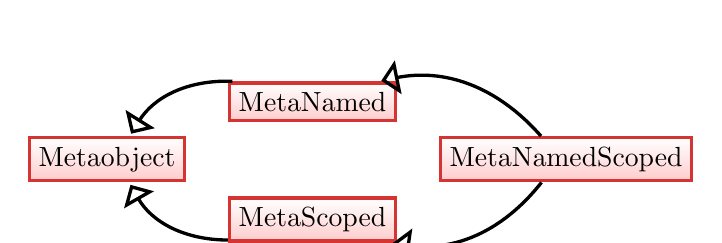
\begin{tikzpicture}
\node [concept] (Metaobject) {Metaobject};
\node [concept] (MetaNamed)[above right=of Metaobject] {MetaNamed}
	edge [inheritance, bend right] (Metaobject);
\node [concept] (MetaScoped)[below right=of Metaobject] {MetaScoped}
	edge [inheritance, bend left] (Metaobject);
\node [concept] (MetaNamedScoped)[below right=of MetaNamed, above right=of MetaScoped] {MetaNamedScoped}
	edge [inheritance, bend right] (MetaNamed)
	edge [inheritance, bend left] (MetaScoped);
\end{tikzpicture}

Models of \meta{NamedScoped} combine the requirements of \meta{Named} and \meta{Scoped}.

\subsection{MetaScope}
\label{concept-MetaScope}

\meta{Scope} is a \meta{NamedScoped} reflecting program constructs defined inside
of a named or anonymous scope (like the global scope, a namespace, a class, etc.)

In addition to the requirements inherited from \meta{NamedScoped}, the following is required:

The \verb@is_scope@ template class specialization for a \meta{Scope} should
inherit from \verb@true_type@:

\begin{minted}{cpp}
template <>
struct is_scope<MetaScope>
 : true_type
{ };
\end{minted}

\subsubsection{\texttt{members}}

A template class \verb@members@ should be defined and should inherit from a
\concept{MetaobjectSequence} containing \meta{NamedScoped} metaobjects reflecting
the members of the base-level scope reflected by this \meta{Scope}.

Furthermore the boolean \verb@All@ parameter (defaulting to \verb@false@ if not specified)
should control which scope members are listed in the resulting metaobject sequence.

If \verb@All@ is 
\begin{itemize}
\item \verb@true@, then all members should be listed,
\item \verb@false@, then the following scope member should {\em not} be included:
	\begin{itemize}
	\item private or protected class members,
	\item scope members with identifiers starting with an underscore followed by a
	(uppercase or lowercase) letter,
	\item scope members annotated by a generalized attributes as hidden (for example
	\verb@[[mirror::hidden]]@ or \verb@[[reflection::hidden]]@).
	\end{itemize}
\end{itemize}



\begin{minted}{cpp}
template <typename T, bool All=false>
struct members;

template <>
struct members<MetaScope, true>
 : MetaobjectSequence<MetaNamedScoped> // all members
{ };

template <>
struct members<MetaScope, false>
 : MetaobjectSequence<MetaNamedScoped> // only 'visible' members
{ };
\end{minted}


\subsection{MetaPositional}
\label{concept-MetaPositional}

\meta{Positional} is a \meta{object}, which is fixed to an ordinal position in some context
usually together with other similar metaobjects, like those reflecting parameters of a function,
or the inheritance of base classes, etc.

In addition to the requirements inherited from \meta{object},
the following must be satisfied:

The \verb@has_position@ template class specialization for a \meta{Positional} should
inherit from \verb@true_type@:

\begin{minted}{cpp}
template <>
struct has_position<MetaPositional>
 : true_type
{ };
\end{minted}

\subsubsection{\texttt{position}}

A template class \verb@position@ should be defined and should
inherit from \verb@integral_constant<size_t, I>@ type where \verb@I@ is
a zero-based position (index) of the reflected base-level language construct,
for example the position of a parameter in a list of function parameters,
or the position of an inheritance clause in the list of base classes.

\begin{minted}{cpp}
template <typename T>
struct position;

template <>
struct position<MetaPositional>
 : integral_constant<size_t, I>
{ };
\end{minted}


\subsection{MetaClassMember}
\label{concept-MetaClassMember}

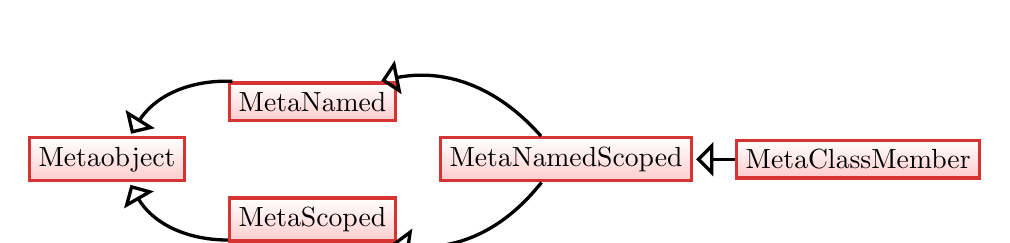
\begin{tikzpicture}
\node [concept] (Metaobject) {Metaobject};
\node [concept] (MetaNamed)[above right=of Metaobject] {MetaNamed}
	edge [inheritance, bend right] (Metaobject);
\node [concept] (MetaScoped)[below right=of Metaobject] {MetaScoped}
	edge [inheritance, bend left] (Metaobject);
\node [concept] (MetaNamedScoped)[below right=of MetaNamed, above right=of MetaScoped] {MetaNamedScoped}
	edge [inheritance, bend right] (MetaNamed)
	edge [inheritance, bend left] (MetaScoped);
\node [concept] (MetaClassMember)[right=of MetaNamedScoped] {MetaClassMember}
	edge [inheritance] (MetaNamedScoped);
\end{tikzpicture}

\meta{Class} is a \meta{Type} and a \meta{Scope} if reflecting a regular class or possibly
also a \meta{Template} if it reflects a class template.

In addition to the requirements inherited from \meta{NamedScoped},
the following is required for \meta{ClassMember}s:

The \verb@is_class_member@ template class specialization for a \meta{ClassMember} should
inherit from \verb@true_type@:

\begin{minted}{cpp}
template <>
struct is_class_member<MetaClassMember>
 : true_type
{ };
\end{minted}

\subsubsection{\texttt{access\_specifier}}

A template class called \verb@access_specifier@ should be defined and should inherit from
a \meta{Specifier} reflecting the \verb@private@, \verb@protected@ or \verb@public@
access specifier:

\begin{minted}{cpp}
template <typename T>
struct access_specifier;

template <>
struct access_specifier<MetaClassMember>
 : MetaSpecifier
{ };
\end{minted}


\subsection{MetaGlobalScope}
\label{concept-MetaGlobalScope}

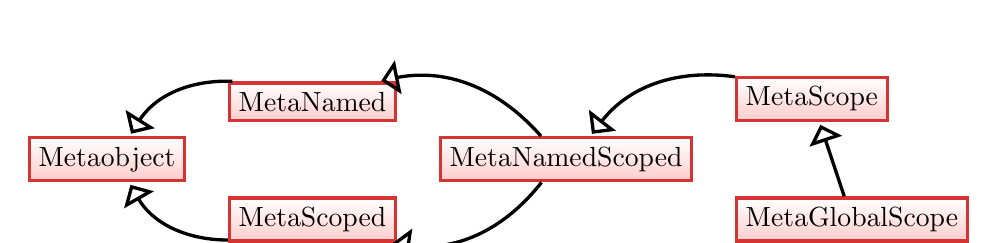
\begin{tikzpicture}
\node [concept] (Metaobject) {Metaobject};
\node [concept] (MetaNamed)[above right=of Metaobject] {MetaNamed}
	edge [inheritance, bend right] (Metaobject);
\node [concept] (MetaScoped)[below right=of Metaobject] {MetaScoped}
	edge [inheritance, bend left] (Metaobject);
\node [concept] (MetaNamedScoped)[below right=of MetaNamed, above right=of MetaScoped] {MetaNamedScoped}
	edge [inheritance, bend right] (MetaNamed)
	edge [inheritance, bend left] (MetaScoped);
\node [concept] (MetaScope)[above right=of MetaNamedScoped] {MetaScope}
	edge [inheritance, bend right] (MetaNamedScoped);
\node [concept] (MetaGlobalScope)[below right=of MetaNamedScoped] {MetaGlobalScope}
	edge [inheritance] (MetaScope);
\end{tikzpicture}

\meta{GlobalScope} is a \meta{Scope} reflecting the global scope.

In addition to the requirements inherited from \meta{Scope}, the following must
be satisfied:

The \verb@metaobject_category@ template class specialization for a \meta{GlobalScope} should
inherit from \verb@global_scope_tag@:

\begin{minted}{cpp}
template <>
struct metaobject_category<MetaNamespace>
 : global_scope_tag
{ };
\end{minted}

The \verb@scope@ template class specialization (required by \meta{Scoped}) for \meta{GlobalScope}
should inherit from the \meta{GlobalScope} itself:

\begin{minted}{cpp}
template <>
struct scope<MetaGlobalScope>
 : MetaGlobalScope
{ };
\end{minted}


\subsection{MetaNamespace}
\label{concept-MetaNamespace}

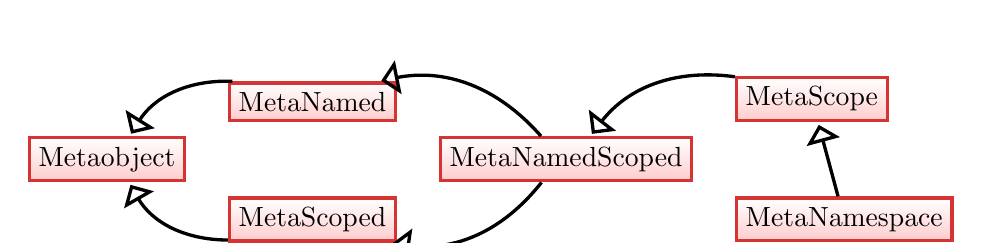
\begin{tikzpicture}
\node [concept] (Metaobject) {Metaobject};
\node [concept] (MetaNamed)[above right=of Metaobject] {MetaNamed}
	edge [inheritance, bend right] (Metaobject);
\node [concept] (MetaScoped)[below right=of Metaobject] {MetaScoped}
	edge [inheritance, bend left] (Metaobject);
\node [concept] (MetaNamedScoped)[below right=of MetaNamed, above right=of MetaScoped] {MetaNamedScoped}
	edge [inheritance, bend right] (MetaNamed)
	edge [inheritance, bend left] (MetaScoped);
\node [concept] (MetaScope)[above right=of MetaNamedScoped] {MetaScope}
	edge [inheritance, bend right] (MetaNamedScoped);
\node [concept] (MetaNamespace)[below right=of MetaNamedScoped] {MetaNamespace}
	edge [inheritance] (MetaScope);
\end{tikzpicture}

\meta{Namespace} is a \meta{Scope} reflecting a namespace.

In addition to the requirements inherited from \meta{Scope}, the following must
be satisfied:

The \verb@metaobject_category@ template class specialization for a \meta{Namespace} should
inherit from \verb@namespace_tag@:

\begin{minted}{cpp}
template <>
struct metaobject_category<MetaNamespace>
 : namespace_tag
{ };
\end{minted}


\subsection{MetaType}
\label{concept-MetaType}

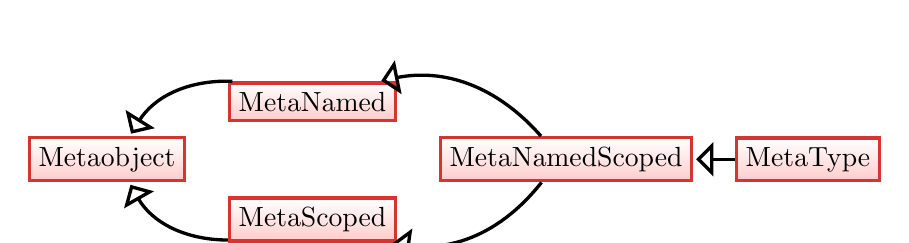
\begin{tikzpicture}
\node [concept] (Metaobject) {Metaobject};
\node [concept] (MetaNamed)[above right=of Metaobject] {MetaNamed}
	edge [inheritance, bend right] (Metaobject);
\node [concept] (MetaScoped)[below right=of Metaobject] {MetaScoped}
	edge [inheritance, bend left] (Metaobject);
\node [concept] (MetaNamedScoped)[below right=of MetaNamed, above right=of MetaScoped] {MetaNamedScoped}
	edge [inheritance, bend right] (MetaNamed)
	edge [inheritance, bend left] (MetaScoped);
\node [concept] (MetaType)[right=of MetaNamedScoped] {MetaType}
	edge [inheritance] (MetaNamedScoped);
\end{tikzpicture}

\meta{Type} is a \meta{NamedScoped} reflecting types.

In addition to the requirements inherited from \meta{NamedScoped}, the following is required:

The \verb@metaobject_category@ template class specialization for a \meta{Type} should
inherit from \verb@type_tag@:

\begin{minted}{cpp}
template <>
struct metaobject_category<MetaType>
 : type_tag
{ };
\end{minted}

\subsubsection{\texttt{original\_type}}

A template class \verb@original_type@ should be defined and should "return"
the original type reflected by this \meta{Type}:

\begin{minted}{cpp}
template <typename T>
struct original_type;

template <>
struct original_type<MetaType>
{
	static_assert(not(is_template<MetaType>::value), "");
	typedef original-type type;
};
\end{minted}

For example, if \verb@__meta_int@ is a metaobject reflecting the \verb@int@ type,
then the specialization of \verb@original_type@ should be following:

\begin{minted}{cpp}
template <>
struct original_type<__meta_int>
{
	typedef int type;
};
\end{minted}

\textbf{Note:} If a concept derived from \meta{Type}, for example a \meta{Class},
is also a \meta{Template} (i.e. is reflecting a template not a concrete type),
then the \verb@original_type@ template should be left undefined.


\subsection{MetaTypedef}
\label{concept-MetaTypedef}

\meta{Typedef} is a \meta{Type} reflecting \verb@typedef@s.

In addition to the requirements inherited from \meta{Type}, the following is required:

The \verb@category@ template class specialization for a \meta{Typedef} should
inherit from \verb@typedef_tag@:

\begin{minted}{cpp}
template <>
struct category<MetaTypedef>
 : typedef_tag
{ };
\end{minted}

\subsubsection{\texttt{decl\_type}}

A template class called \verb@decl_type@ should be defined and should inherit from the \meta{Type}
reflecting the "source" type of the typedef:

\begin{minted}{cpp}
template <typename T>
struct decl_type;

template <>
struct decl_type<MetaTypedef>
 : MetaType
{ };
\end{minted}

For example if \verb@__meta_std_string@ is a \meta{Typedef} reflecting the \verb@std::string@
typedef and \verb@__meta_std_basic_string_char@ is the \meta{Type} that reflects
the \verb@std::basic_string<char>@ type, and \verb@std::string@ is defined as:

\begin{minted}{cpp}
namespace std {
typedef basic_string<char> string;
}
\end{minted}

then the specialization of \verb@decl_type@ for \verb@__meta_std_string@ should be following:

\begin{minted}{cpp}
template <>
struct decl_type<__meta_std_string>
 : __meta_std_basic_string_char
{ };
\end{minted}

\textbf{Note:} If this feature proves to be too difficult to implement 
at this point\footnote{since some compilers do not keep typedef information},
it can be added later. We, however, think that leaving it out completely would
seriously limit the utility of reflection in certain use cases.

\subsection{MetaClass}
\label{concept-MetaClass}

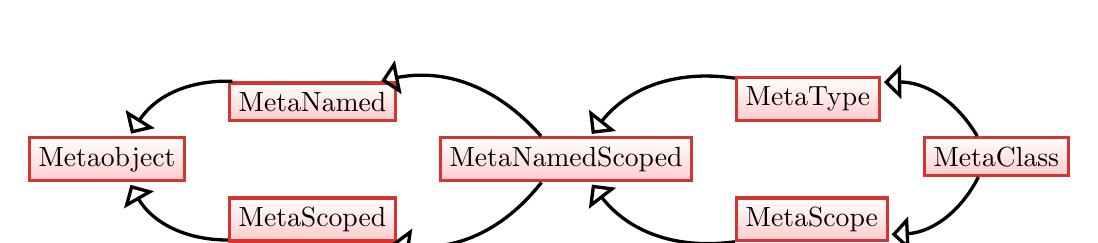
\begin{tikzpicture}
\node [concept] (Metaobject) {Metaobject};
\node [concept] (MetaNamed)[above right=of Metaobject] {MetaNamed}
	edge [inheritance, bend right] (Metaobject);
\node [concept] (MetaScoped)[below right=of Metaobject] {MetaScoped}
	edge [inheritance, bend left] (Metaobject);
\node [concept] (MetaNamedScoped)[below right=of MetaNamed, above right=of MetaScoped] {MetaNamedScoped}
	edge [inheritance, bend right] (MetaNamed)
	edge [inheritance, bend left] (MetaScoped);
\node [concept] (MetaType)[above right=of MetaNamedScoped] {MetaType}
	edge [inheritance, bend right] (MetaNamedScoped);
\node [concept] (MetaScope)[below right=of MetaNamedScoped] {MetaScope}
	edge [inheritance, bend left] (MetaNamedScoped);
\node [concept] (MetaClass)[below right=of MetaType] {MetaClass}
	edge [inheritance, bend right] (MetaType)
	edge [inheritance, bend left] (MetaScope);
\end{tikzpicture}

\meta{Class} is a \meta{Type} and a \meta{Scope} if reflecting a regular class or possibly
also a \meta{Template} if it reflects a class template.

In addition to the requirements inherited from \meta{Type}, \meta{Scope}
and optionally from \meta{Template},
models of \meta{Class} are subject to the following:

The \verb@metaobject_category@ template class specialization for a \meta{Class} should
inherit from \verb@class_tag@:

\begin{minted}{cpp}
template <>
struct metaobject_category<MetaClass>
 : class_tag
{ };
\end{minted}

If a \meta{Class} reflects a class template, then the \verb@is_template@
trait should inherit from \verb@true_type@

\subsubsection{\texttt{elaborated\_type\_specifier}}

A template class called \verb@elaborated_type_specifier@ should be defined and should inherit from
a \meta{Specifier} reflecting the \verb@class@, \verb@struct@ or \verb@union@
specifiers:

\begin{minted}{cpp}
template <typename T>
struct elaborated_type_specifier;

template <>
struct elaborated_type_specifier<MetaClass>
 : MetaSpecifier
{ };
\end{minted}

\subsubsection{\texttt{base\_classes}}

A template class \verb@base_classes@ should be defined and should inherit from
a \concept{MetaobjectSequence} of \meta{Inheritance}s, each one of which reflects the inheritance
of a single base class of the class reflected by the \meta{Class}:

\begin{minted}{cpp}
template <typename T>
struct base_classes;

template <>
struct base_classes<MetaClass>
 : MetaobjectSequence<MetaInheritance>
{ };
\end{minted}


\subsection{MetaInheritance}
\label{concept-MetaInheritance}

\meta{Inheritance} is a \meta{Scoped} and \meta{Positional} reflecting class inheritance.

In addition to the requirements inherited from \meta{Scoped} and \meta{Positional},
types conforming to this concept must satisfy the following:

The \verb@category@ template should return \verb@inheritance_tag@ for models
of \meta{Inheritance}:

\begin{minted}{cpp}
template <>
struct category<MetaInheritance>
 : inheritance_tag
{ };
\end{minted}

The \verb@scope@ member function should inherit from a \meta{Class} reflecting
the derived class in the inheritance:

\begin{minted}{cpp}
template <>
struct scope<MetaInheritance>
 : MetaClass
{ };
\end{minted}

\subsubsection{\texttt{access\_specifier}}

A template struct \verb@access_specifier@ should be defined and should inherit from
a \meta{Specifier} reflecting one of the \verb@private@, \verb@protected@ and
\verb@public@ access specifiers.

\begin{minted}{cpp}
template <typename T>
struct access_specifier;

template <>
struct access_specifier<MetaInheritance>
 : MetaSpecifier
{ };
\end{minted}

\subsubsection{\texttt{inheritance\_specifier}}

A template struct \verb@inheritance_specifier@ should be defined and should inherit from
a \meta{Specifier} reflecting one of the \verb@virtual@ and "none" access specifiers.

\begin{minted}{cpp}
template <typename T>
struct inheritance_specifier;

template <>
struct inheritance_specifier<MetaInheritance>
 : MetaSpecifier
{ };
\end{minted}

\subsubsection{\texttt{base\_class}}

A template struct \verb@base_class@ should be defined and should inherit from
a \meta{Class} reflecting the base class in the inheritance:

\begin{minted}{cpp}
template <typename T>
struct base_class;

template <>
struct base_class<MetaInheritance>
 : MetaClass
{ };
\end{minted}


\subsection{MetaVariable}
\label{concept-MetaVariable}

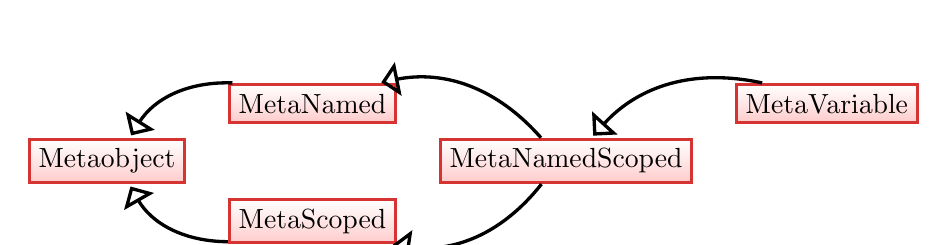
\begin{tikzpicture}
\node [concept] (Metaobject) {Metaobject};
\node [concept] (MetaNamed)[above right=of Metaobject] {MetaNamed}
	edge [inheritance, bend right] (Metaobject);
\node [concept] (MetaScoped)[below right=of Metaobject] {MetaScoped}
	edge [inheritance, bend left] (Metaobject);
\node [concept] (MetaNamedScoped)[below right=of MetaNamed, above right=of MetaScoped] {MetaNamedScoped}
	edge [inheritance, bend right] (MetaNamed)
	edge [inheritance, bend left] (MetaScoped);
\node [concept] (MetaVariable)[above right=of MetaNamedScoped] {MetaVariable}
	edge [inheritance, bend right] (MetaNamedScoped);
\end{tikzpicture}

\meta{Variable} is a \meta{NamedScoped} reflecting a variable.

In addition to the requirements inherited from \meta{NamedScoped}, the following must
be satisfied:

The \verb@metaobject_category@ template class specialization for a \meta{Variable} should
inherit from \verb@variable_tag@:

\begin{minted}{cpp}
template <>
struct metaobject_category<MetaVariable>
 : variable_tag
{ };
\end{minted}

\subsubsection{\texttt{storage\_specifier}}

A template class \verb@storage_specifier@ should be added and should
inherit from a \meta{Specifier} reflecting a storage class specifier:

\begin{minted}{cpp}
template <typename T>
struct storage_specifier;

template <>
struct storage_specifier<MetaVariable>
 : MetaSpecifier
{ };
\end{minted}

\subsubsection{\texttt{type}}

A template class \verb@type@ should be added and should inherit
from a \meta{Type} reflecting the type of the variable:

\begin{minted}{cpp}
template <typename T>
struct type;

template <>
struct type<MetaVariable>
 : MetaType
{ };
\end{minted}

\subsubsection{\texttt{pointer}}

If the reflected variable is a namespace-level variable, then a template
class \verb@pointer@ should be implemented as follows:

\begin{minted}{cpp}
template <typename T>
struct pointer;

template <>
struct pointer<MetaVariable>
{
	typedef typename original_type<type<MetaVariable>>::type* type;

	static type get(void);
};
\end{minted}

The static member function \verb@get@ should return the address of the reflected variable.

If the reflected variable is a class member variable (i.e. if the \meta{Variable}
is also a \meta{ClassMember}), then the \verb@pointer@ template class should be
defined as follows:

\begin{minted}{cpp}

template <>
struct pointer<MetaVariable>
{
	typedef typename original_type<type<MetaVariable>>::type
		_mv_t;
	typedef typename original_type<type<scope<MetaVariable>>>::type
		_cls_t;

	typedef _mv_t _cls_t::* type;

	static type get(void);
};

\end{minted}

The static member function \verb@get@ should return a data member pointer to
the reflected member variable. The \verb@_mv_t@ and \verb@_cls_t@ typedefs
are implementation details and are not a part of this specification.


\section{Reflection operator}

The metaobjects reflecting some program feature \verb@X@ as
described above should be made available to the user by
the means of a new operator or expression.
More precisely, the reflection operator should return a type conforming to a particular
metaobject concept, depending on the reflected expression.

Since adding a new keyword has the potential to break existing code,
we do not insist on any particular expression, here follows a list of suggestions
in order of preference (from the most to the least preferrable):

\begin{itemize}
\item{\verb@mirrored(X)@}
\item{\verb@reflected(X)@}
\item{\verb@reflexpr(X)@}
\item{\verb@|X@}
\item{\verb@[[X]]@}
\item{\verb@<<X>>@}
\end{itemize}

The reflected expression \verb@X@ in the items listed above can be any of the following:

\begin{itemize}
\item{\verb@::@} -- The global scope, the returned metaobject is a {\meta{GlobalScope}}.
\item{{\em Namespace name}} -- (\verb@std@) the returned metaobject is a {\meta{Namespace}}.
\item{{\em Type name}} -- (\verb@long double@) the returned metaobject is a {\meta{Type}}.
\item{{\em \verb@typedef@ name}} -- (\verb@std::size_t@ or \verb@std::string@)
     the returned metaobject is a {\meta{Typedef}}.
\item{{\em Template name}} -- (\verb@std::tuple@ or \verb@std::map@)
     the returned metaobject is a {\meta{Template}}.
\item{{\em Class name}} -- (\verb@std::thread@ or \verb@std::map<int, double>@)
     the returned metaobject is a {\meta{Class}}.
\item{{\em Function name}} -- (\verb@std::sin@ or \verb@std::string::size@) the returned metaobject
     is a {\meta{OverloadedFunction}}.
\item{{\em Function signature}} -- (\verb@std::sin(double)@ or \verb@std::string::front(void) const@)
     the returned metaobject is a {\meta{Function}}. The signature may be specified without the
     return value type.
\item{{\em Constructor signature}} -- (\verb@std::pair<char, double>::pair(char, double)@
     or \verb@std::string::string(void)@) the returned metaobject is a {\meta{Constructor}}.
\item{{\em Variable name}} -- (\verb@std::errno@) the returned metaobject is a {\meta{Variable}}.
%\item{TODO}
\end{itemize}

The reflection operator or expression should have access to \verb@private@ and
\verb@protected@ members of classes. The following should be valid:

\begin{minted}{cpp}
struct A
{
	int a;
};

class B
{
protected:
	int b;
};

class C
 : protected A
 , public B
{
private:
	int c;
};

typedef mirrored(A::a) meta_A_a;
typedef mirrored(B::b) meta_B_b;
typedef mirrored(C::a) meta_C_a;
typedef mirrored(C::b) meta_C_b;
typedef mirrored(C::c) meta_C_c;

\end{minted}

\subsection{Context-dependent reflection}

We also propose to define a set of special expressions that can be used
inside of the reflection operator, to obtain metadata based on the context
where it is invoked, instead of the identifier.

\subsubsection{Namespaces}

If the \verb@this::namespace@ expression is used as the argument of the reflection
operator, then it should return a \meta{Namespace} reflecting the namespace
inside of which the reflection operator was invoked.

For example:

\begin{minted}{cpp}

typedef mirrored(this::namespace) _meta_gs;

\end{minted}

reflects the global scope namespace and is equivalent to

\begin{minted}{cpp}

typedef mirrored(::) _meta_gs;

\end{minted}

For named namespaces:

\begin{minted}{cpp}

namespace foo {

typedef mirrored(this::namespace) _meta_foo;

namespace bar {

typedef mirrored(this::namespace) _meta_foo_bar;

} // namespace bar

} // namespace foo
\end{minted}

\subsubsection{Classes}

If the \verb@this::class@ expression is used as the argument of the reflection
operator, then it should return a \meta{Class} reflecting the class
inside of which the reflection operator was invoked.

For example:

\begin{minted}{cpp}

struct foo
{
	const char* _name;

	// reflects foo
	typedef mirrored(this::class) _meta_foo1;

	foo(void)
	 : _name(base_name<mirrored(this::class)>())
	{ }

	void f(void)
	{
		// reflects foo
		typedef mirrored(this::class) _meta_foo2;
	}

	double g(double, double);

	struct bar
	{
		// reflects foo::bar
		typedef mirrored(this::class) _meta_foo_bar;
	};
};

double foo::g(double a, double b)
{
	// reflects foo
	typedef mirrored(this::class) _meta_foo3;
	return a+b;
}

class baz
{
private:
	typedef mirrored(this::class) _meta_baz;
};

typedef mirrored(this::class); // <- error: not used inside of a class.

\end{minted}

\subsubsection{Functions}

If the \verb@this::function@ expression is used as the argument of the reflection
operator, then it should return a \meta{Function} reflecting the function or operator
inside of which the reflection operator was invoked.

For example:

\begin{minted}{cpp}

void foobar(void)
{
	// reflects this particular overload of the foobar function
	typedef mirrored(this::function) _meta_foobar;
}

int foobar(int i)
{
	// reflects this particular overload of the foobar function
	typedef mirrored(this::function) _meta_foobar;
	return i+1;
}

class foo
{
private:
	void f(void)
	{
		// reflects this particular overload of foo::f
		typedef mirrored(this::function) _meta_foo_f;
	}

	double f(void)
	{
		// reflects this particular overload of foo::f
		typedef mirrored(this::function) _meta_foo_f;
		return 12345.6789;
	}
public:
	foo(void)
	{
		// reflects this constructor of foo
		typedef mirrored(this::function) _meta_foo_foo;
	}

	friend bool operator == (foo, foo)
	{
		// reflects this operator
		typedef mirrored(this::function) _meta_foo_eq;
	}

	typedef mirrored(this::function) _meta_fn; // <- error
};

typedef mirrored(this::function) _meta_fn; // <- error

\end{minted}


\section{Additions to the library}
\label{section-Library}

In order to simplify composition of the metaobjects and metafunctions defined
\hyperref[section-Concepts]{above}, several further additions to the standard
library should be made.

\subsection{Metaobject expressions}

A {\em metaobject expression} is a class which can be {\em evaluated}
into a \meta{object}. By default any class, that has a member typedef
called \verb@type@, which is a model of \meta{object}, is a metaobject expression.

\begin{minted}{cpp}
struct SomeMetaobjectExpression
{
	typedef Metaobject type;
};

\end{minted}

And thus, any \meta{object} is also a {\em metaobject expression}.

Generally, however, any type for which the \verb@evaluate@ metafunction
(described below), "returns" a \meta{object} is a {\em metaobject expression}.

\subsubsection{\texttt{evaluate}}

A class template called \verb@evaluate@ should be defined and should "return" a \meta{object}
resulting from a {\em metaobject expression}:

\begin{minted}{cpp}
template <class MetaobjectExpression>
struct evaluate
 : Metaobject
{ };
\end{minted}

that could be implemented for example as follows:

\begin{minted}{cpp}
template <class X, bool IsMetaobject>
struct do_evaluate;

template <class X>
struct do_evaluate<X, true>
 : X
{ };

template <class X>
struct do_evaluate<X, false>
 : do_evaluate<
	typename X::type,
	is_metaobject<typename X::type>::value
> { };

template <class X>
struct evaluate
 : do_evaluate<X, is_metaobject<X>::value>
{ };

\end{minted}

The users should be allowed to add specializations of \verb@evaluate@
for other types if necessary.

\subsection{Default implementation of metafunctions}

The default implementation of the metafunction template classes defined above,
should follow this pattern:

\begin{minted}{cpp}
template <typename T>
struct Template;

template <typename T>
struct Template
 : Template<typename evaluate<T>::type>
{ };
\end{minted}

Where \verb@Template@ is each of the following:

\begin{minipage}[t]{0.5\textwidth}
\begin{itemize}
\item \verb@metaobject_category@
\item \verb@specifier_category@
\item \verb@keyword@
\item \verb@base_name@
\item \verb@full_name@
\item \verb@named_typedef@
\item \verb@named_mem_var@
\item \verb@scope@
\item \verb@members@
\item \verb@overloads@
\item \verb@type@
\item \verb@base_classes@
\item \verb@base_class@
\item \verb@base_type@
\item \verb@result_type@
\item \verb@parameters@
\item \verb@template_parameters@
\end{itemize}
\end{minipage}
\begin{minipage}[t]{0.5\textwidth}
\begin{itemize}
\item \verb@template_arguments@
\item \verb@template_@
\item \verb@exceptions@
\item \verb@instantiation@
\item \verb@position@
\item \verb@value@
\item \verb@elaborated_type_specifier@
\item \verb@access_specifier@
\item \verb@constexpr_specifier@
\item \verb@noexcept_specifier@
\item \verb@const_specifier@
\item \verb@inheritance_specifier@
\item \verb@linkage_specifier@
\item \verb@storage_specifier@
\item \verb@is_pure@
\item \verb@is_pack@
\item \verb@original_type@
\end{itemize}
\end{minipage}

For example:

\begin{minted}{cpp}
template <typename T>
struct metaobject_category
 : metaobject_category<typename evaluate<T>::type>
{ };
\end{minted}

This will allow to compose metaobject expressions into algorithms. For example:

\begin{minted}[tabsize=4]{cpp}
// print the number of members of the scope where mycls is defined
cout << size<members<scope<mirrored(mycls)>>>() << endl;

// print the name of the first base class of mycls
cout <<
	base_name<base_class<at<base_classes<mirrored(mycls)>, 0>>>()
<< endl;

// print the access specifier keyword of the second base of mycls
cout <<
	keyword<access_specifier<at<base_classes<mirrored(mycls)>, 1>>>()
<< endl;

// print the fully qualified name of the scope of
// the source type of the third member of mycls
cout <<
	full_name<scope<type<at<members<mirrored(mycls)>, 2>>>>()
<< endl;
\end{minted}


\section{Rationale}

This section explains some of the design decisions behind this proposal and
answers several frequently asked questions.

\subsection{Why metaobjects, why not reflect directly?}

{\textbf Q:}{\em Why should we define a set of metaobject concepts, let the compiler generate
models of these concepts and use those to obtain the metadata? Why not just extend the existing
type traits?}

{\textbf A:} The most important reason is the completeness and the scope of reflection.
Type traits (as they are defined now) work just with types. A reflection facility should
however provide much more metadata.
It should be able to reflect namespaces, functions, constructors, inheritance, variables, etc.

For example:

\begin{minted}{cpp}
pair<long, string> my_var;

// OK, we can print the name of the type of a variable:
cout << type_name<decltype(my_var)>() << endl;
// But we really, really want to print the name of the variable
// (without the use of the preprocessor)
cout << type_name<my_var>() << endl; // Error
// similar with namespaces:
cout << type_name<std::chrono>() << endl; // Error
// etc.
\end{minted}


Doing reflection with type traits limits the scope, because of the rules defining what
can be a template parameter. This rules could be updated to allow for example an expression
representing a particular class constructor to  be passed as a template argument.
Also currently there is no expression for specifying (not invoking) a constructor
or a particular function overload, so additional rules would have to be added.

This would (in our opinion) be a much more drastic change to the standard, than
the adoption of this proposal. If expressions denoting a namespace or a particular
constructor or a function overload were added just for the purpose of reflecting
them (with the \verb@mirroed@ keyword), then all the changes could be localized
in the reflection subsystem and remain invalid in the core language:

\begin{minted}{cpp}
mirrored(std::current_thread); // OK - MetaNamespace
std::current_thread; // error - not a primary expression

mirrored(std::sin); // OK - MetaOverloadedFunction
std::sin; // error - cannot resolve overload

mirrored(std::sin(double)); // OK - MetaFunction
std::sin(double); // error - invalid expression
//etc.
\end{minted}


Second reason is access to private and protected members. There are many use-cases where
access to non-public class members through reflection is desired. If reflection was
done through type traits directly on the class members, it would be either impossible
to reflect non-public members or the access rules would have to be changed to somehow
allow access in reflection expressions:

\begin{minted}{cpp}
class C
{
private:
	typedef int T;
public:
};

assert(some_trait<C::T>::value); //OK, we are reflecting so we have access
\end{minted}

but not outside:

\begin{minted}{cpp}
C::T x = 0; // Error, C::T is private
\end{minted}

With the reflection operator like \verb@mirrored(X)@, the access rules would have
to be updated only to allow the reflection operator to have access to everthing.
At the first glance, the following two expressions;

\begin{minted}{cpp}
some_trait<C::T>::value
\end{minted}

and

\begin{minted}{cpp}
mirrored(C::T)
\end{minted}

look similar and so the changes to the access rules could seem similar too, but
that is not the case. The (single) \verb@mirrored@ operator would have special status,
on the other hand type traits are regular templates (with some magic inside) and
all (several dozens of them) would need to be distinguished from all the other templates
in the \verb@std@ namespace, which should not have private access.

Having said that, we do not object to extending the type traits where it does make sense.

One other reason for having a new reflection operator is, that there already is an
existing (very limited) reflection operator, namely \verb@typeid@ which "returns"
a compiler-generated "metaobject" -- \verb@std::type_info@. We are aware that there
are differences between \verb@typeid@ and \verb@mirrored@, but the basic idea is similar.

\subsection{Why are the metaobjects anonymous?}

{\textbf Q:}{\em Why should the metaobjects be anonymous types as opposed to
types with well defined and standardized names or concrete template classes, (possibly with some
special kind of parameter accepting different arguments than types and constants)?}

{\textbf A:} We wanted to avoid defining a specific naming convention, because it would
be difficult to do so and very probably not user friendly (see C++ name mangling). There
already is a precedent for anonymous types -- for example C++ {\em lambdas}.

Another option would be to define a concrete set of template classes like:

\begin{minted}{cpp}
namespace std {

template <typename T>
class meta_type /* Model of MetaType */
{ };

}
\end{minted}

which could work with types, classes, etc., but would not work with namespaces, constructors,
etc. (see also the Q/A above):

\begin{minted}{cpp}
namespace std {

template <something X> //<- Problem
class meta_constructor /* Model of MetaConstructor */
{ };

template <something X> //<- Problem
class meta_namespace /* Model of MetaNamespace */
{ };

}

typedef std::meta_namespace<std> meta_std; //<- Problem
\end{minted}

Instead of this, the metaobjects are anonymous and their (internal) identification
is left to the compiler. From the users POV, the metaobject can be distinguished
by the means of the metaobject traits and tags as \hyperref[section-Concepts]{described above}.

\section{Unresolved Issues}

\begin{itemize}
	\item {\em Normalization of names returned by \verb@Named::base_name()@ and \verb@Named::full_name()@:}
	The strings returned by the \verb@base_name@ and \verb@full_name@ functions should be
	implementation-independent and the same on every platform/compiler.
	

	\item {\em Returning names as compile-time strings:} It could be advantageous if even
	the names of various metaobjects were compile-time constants and could be introspected
	or used as template parameters.
\end{itemize}

\section{Acknowledgements}

Thanks to Chandler Carruth for presenting the N4111 proposal at the Urbana meeting.
Also thanks to Axel Naumann for helping with this proposal.


\renewcommand\refname{\arabic{section}\hspace{1em}References}

\stepcounter{section}
\addcontentsline{toc}{section}{\refname}

\begin{thebibliography}{100}

\bibitem{mirror-doc-cpp11}
Mirror C++ reflection library documentation (C++11 version),
\url{http://kifri.fri.uniza.sk/~chochlik/mirror-lib/html/}.

\end{thebibliography}{100}



\begin{appendices}
\appendix
\section{All metaobject concepts}
\label{section-all-Concepts}

In order to keep the big picture in mind, this section
contains the descriptions of all metaobject concepts
including their full interfaces as they are envisioned
to look when reflection is fully implemented. We
however {\em do not} propose to implement them at this moment.

TODO

%\subsection{Metaobject Sequence}
\label{concept-MetaobjectSequence}

As the name implies \concept{MetaobjectSequence}s are used to store seqences
or tuples of metaobjects.
A model of \concept{MetaobjectSequence} is a class conforming to the following:

It is a nullary metafunction returning itself:

\begin{minted}{cpp}
template <typename Metaobject>
struct MetaobjectSequence
{
	typedef MetaobjectSequence type;
};
\end{minted}

\textbf{Note:} The definition above is only a psedo-code and
the template parameter \verb@Metaobject@ indicates here the minimal
metaobject concept which all elements in the sequence must satisfy.
For example a \verb@MetaobjectSequence<MetaConstructor>@ denotes a sequence
of metaobjects that all satisfy the \meta{Constructor} concept, etc.

\subsubsection{\texttt{size}}

A template class \verb@size@ is defined as follows:

\begin{minted}{cpp}
template <typename T>
struct size;

template <>
struct size<MetaobjectSequence<Metaobject>>
 : integral_type<size_t, N>
{ };
\end{minted}

Where \verb@N@ is the number of elements in the sequence.

\subsubsection{\texttt{at}}

A template class \verb@at@, providing random access to metaobjects in a sequence
is defined (for values of \verb@I@ between \verb@0@ and \verb@N-1@ where \verb@N@
is the number of elements returned by \verb@size@) as follows:

\begin{minted}{cpp}
template <typename T, size_t I>
struct at;

template <size_t I>
struct at<MetaobjectSequence<Metaobject>, I>
 : Metaobject
{ };
\end{minted}

For example if \verb@__meta_seq_ABC@ is a metaobject sequence containing three metaobjects;
\verb@__meta_A@, \verb@__meta_B@ and \verb@__meta_C@ (in that order), then:

\begin{minted}{cpp}
template <>
struct size<__meta_seq_ABC>
 : integral_constant<size_t, 3>
{ };
\end{minted}

and 

\begin{minted}{cpp}
template <>
struct at<__meta_seq_ABC, 0>
 : __meta_A
{ };

template <>
struct at<__meta_seq_ABC, 1>
 : __meta_B
{ };

template <>
struct at<__meta_seq_ABC, 2>
 : __meta_C
{ };
\end{minted}

\textbf{Note:} The order of the metaobjects in a sequence is determined by the order
of appearance in the processed translation unit.

\subsubsection{\texttt{for\_each}}

A template function \verb@for_each@ should be defined and should
execute the specified unary function on every \meta{object} in
the sequence, in the order of appearance in the processed translation unit.

\begin{minted}{cpp}
template <typename MetaobjectSequence, typename UnaryFunc>
void for_each(UnaryFunc func)
{
	func(Metaobject1());
	func(Metaobject2());
	/* ... */
	func(MetaobjectN());
}

\end{minted}

This design requires the metaobjects to be default constructible.
If this should prove to be a problem then an \verb@identity@ wrapper could be used
instead:

\begin{minted}{cpp}
template <typename X>
struct identity
{
	typedef X type;
};

template <typename MetaobjectSequence, typename UnaryFunc>
void for_each(UnaryFunc func)
{
	func(identity<Metaobject1>());
	func(identity<Metaobject2>());
	/* ... */
	func(identity<MetaobjectN>());
}

\end{minted}

\textbf{Note:} The interface of \meta{objectSequence}, in particular \verb@size@
and \verb@at@ together with \verb@std::index_sequence@ should be enough
to implement a single generic version of \verb@for_each@.


%\subsection{Metaobject}
\label{concept-Metaobject}

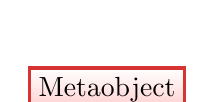
\begin{tikzpicture}
\node[concept] (Metaobject) {Metaobject};
\end{tikzpicture}

A \meta{object} is a stateless anonymous type generated by the compiler which
provides metadata reflecting a specific program feature. Each metaobject
should satisfy the following:

Every metaobject should be a nullary metafunction returning itself:

\begin{minted}{cpp}
struct Metaobject
{
	typedef Metaobject type;
};
\end{minted}

One possible way how to achieve this is to define {\em basic metaobjects}
as plain types (without any internal structure) and define a class template like:

\begin{minted}{cpp}
template <typename BasicMetaobject>
struct metaobject
{
	typedef metaobject type;
};
\end{minted}

and then, implement the actual \meta{object}s as instantiations of this template.
For example if \verb@__base_meta_int@ is a basic metaobject reflecting the \verb@int@
type then the actual metaobject \verb@__meta_int@ conforming to this concept could 
be defined as:

\begin{minted}{cpp}
typedef metaobject<__base_meta_int> __meta_int;
\end{minted}

Although, this is just one possibility not a requirement of this proposal.

\subsubsection{\texttt{is\_metaobject}}

The \verb@is_metaobject@ template should inherit from \verb@true_type@ for all \meta{object}s,
and inherit from \verb@false_type@ otherwise.

\begin{minted}{cpp}
template <typename T>
struct is_metaobject
 : false_type
{ };

template <>
struct is_metaobject<Metaobject>
 : true_type
{ };
\end{minted}

\subsubsection{\texttt{metaobject\_category}}

A template class \verb@metaobject_category@ should be defined in the \verb@std@ namespace
(even if everything else is defined inside of a nested namespace like \verb@std::meta@)
and should inherit from
one of the \hyperref[metaobject-category-tags]{metaobject category tags}, depending on
the actual kind of the metaobject.

\begin{minted}{cpp}
template <typename T>
struct metaobject_category;

template <>
struct metaobject_category<Metaobject>
 : MetaobjectCategory
{ };
\end{minted}

For example if the \verb@__meta_std@ metaobject reflects the \verb@std@ namespace,
then the specialization of \verb@metaobject_category@ should be:

\begin{minted}{cpp}
template <>
struct metaobject_category<__meta_std>
 : namespace_tag
{ };
\end{minted}

\subsubsection{Comparison}

A template class \verb@equal@ should be defined and should inherit from \verb@true_type@
if a \hyperref[section-Library]{metaobject expression} \verb@Expr1@ {\em evaluates} into
the same metaobject as the metaobject expression \verb@Expr2@ (i.e. into metaobjects
that both reflect the same base-level construct). Otherwise it should inherit from
\verb@false_type@:

\begin{minted}{cpp}
template <typename Expr1, typename Expr2>
struct equal
 : BooleanConstant
{ };
\end{minted}

\subsubsection{Traits}

The following template classes indicating various properties of a \meta{object}
should be defined and should by default inherit from \verb@false_type@ unless stated
otherwise below:

\verb@has_name@ -- indicates that a \meta{object} is a \meta{Named}:
\begin{minted}{cpp}
template <typename T>
struct has_name
 : false_type
{ };
\end{minted}

\verb@has_scope@ -- indicates that a \meta{object} is a \meta{Scoped}:
\begin{minted}{cpp}
template <typename T>
struct has_scope
 : false_type
{ };
\end{minted}

\verb@is_scope@ -- indicates that a \meta{object} is a \meta{Scope}:
\begin{minted}{cpp}
template <typename T>
struct is_scope
 : false_type
{ };
\end{minted}

\verb@has_name@ -- indicates that a \meta{object} is a \meta{Positional}:
\begin{minted}{cpp}
template <typename T>
struct has_position
 : false_type
{ };
\end{minted}

\verb@is_class_member@ -- indicates that a \meta{object} is a \meta{ClassMember}:
\begin{minted}{cpp}
template <typename T>
struct is_class_member
 : false_type
{ };
\end{minted}

\verb@has_template@ -- indicates that a \meta{object} is a \meta{Instantiation}:
\begin{minted}{cpp}
template <typename T>
struct has_template
 : false_type
{ };
\end{minted}

\verb@is_template@ -- indicates that a \meta{object} is a \meta{Template}
or \meta{TemplateParameter}:
\begin{minted}{cpp}
template <typename T>
struct is_template
 : false_type
{ };
\end{minted}

\subsubsection{\texttt{source\_file}}

A template class \verb@source_file@ should be defined and should return the
path to the source file where the base-level construct reflected by a
metaobject is defined (similar to what the preprocessor \verb@__FILE__@ macro
expands to).

\begin{minted}{cpp}
template <typename T>
struct source_file;

template <>
struct source_file<MetaObject>
 : StringConstant
{ };
\end{minted}

For base-level constructs like namespaces which don't have a single specific
declaration, an empty string should be returned.

\subsubsection{\texttt{source\_line}}

A template class \verb@source_line@ should be defined and should return the (positive)
line number in the source file where the base-level construct reflected by a
metaobject is defined (similar to what the preprocessor \verb@__LINE__@ symbol
expands to).

\begin{minted}{cpp}
template <typename T>
struct source_line;

template <>
struct source_line<MetaObject>
 : integral_constant<unsigned, Line>
{ };
\end{minted}

For base-level constructs like namespaces which don't have a single specific
declaration, line number zero should be returned.


%\subsection{MetaSpecifier}
\label{concept-MetaSpecifier}

\meta{Specifier} is a \meta{object} reflecting a C++ specifier. There also should be a "none"
\meta{Specifier} reflecting a missing specifier. For example the \verb@const@ specifier
on member functions can be either specified or not. In the latter case this "none" \meta{Specifier}
should be "returned".


In addition to the requirements inherited from \meta{object}, types conforming to this concept
must satisfy the following:

The \verb@category@ template should return \verb@specifier_tag@ for all \meta{Specifier}s.

\begin{minted}{cpp}
template <>
struct category<MetaSpecifier>
 : specifier_tag
{ };
\end{minted}

\subsubsection{\texttt{category}}

A template struct \verb@category@ should be defined and should inherit from one of the
\hyperref[specifier-category-tags]{specifier category tags}, depending on
the actual reflected specifier.

\begin{minted}{cpp}
template <typename T>
struct category;

template <>
struct category<MetaSpecifier>
 : SpecifierCategory
{ };
\end{minted}

For example if the \verb@__meta_static@ metaobject reflects the \verb@static@
C++ specifier, then the specialization of \verb@category@
should be:

\begin{minted}{cpp}
template <>
struct category<__meta_static>
 : static_tag
{ };
\end{minted}

If \verb@__meta_nospec@ is the \meta{Specifier} reflecting the "none" (missing) specifier,
then the specialization of \verb@category@ should be:

\begin{minted}{cpp}
template <>
struct category<__meta_nospec>
 : none_tag
{ };
\end{minted}


\subsubsection{\texttt{keyword}}

A template struct \verb@keyword@ should be defined and should return
the keyword matching the reflected specifier as a
\concept{StringConstant}.

\begin{minted}{cpp}
template <typename T>
struct keyword;

template <>
struct keyword<MetaSpecifier>
 : StringConstant
{ };
\end{minted}

For example if the \verb@__meta_thread_local@ metaobject reflects the \verb@thread local@
specifier, then the matching specialization of \verb@keyword@ could be following:

\begin{minted}{cpp}
template <>
struct keyword<__meta_thread_local>
 : string_constant<'t','h','r','e','a','d',' ','l','o','c','a','l'>
{ };
\end{minted}

If \verb@__meta_nospec@ is the \meta{Specifier} reflecting the "none" (missing) specifier,
then the specialization of \verb@keyword@ should return an empty string constant.
For example:

\begin{minted}{cpp}
template <>
struct keyword<__meta_nospec>
 : string_constant<>
{ };
\end{minted}

The \verb@string_constant<'t','h','r','e','a','d',' ','l','o','c','a','l'>@
and the \verb@string_constant<>@ classes should be models of \concept{StringConstant}
as described above.


%\subsection{MetaNamed}
\label{concept-MetaNamed}

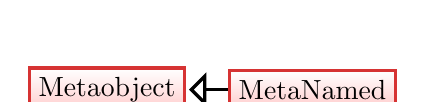
\begin{tikzpicture}
\node[concept] (Metaobject) {Metaobject};
\node[concept] (MetaNamed) [right=of Metaobject] {MetaNamed}
	edge[inheritance] (Metaobject);
\end{tikzpicture}

\meta{Named} is a \meta{object} reflecting program constructs, which have a name
(are identified by an identifier) like namespaces, types, functions, variables, parameters, etc.

In addition to the requirements inherited from \meta{object}, the following requirements must
be satisfied:

The \verb@has_name@ template class specialization for a \meta{Named} should
inherit from \verb@true_type@:

\begin{minted}{cpp}
template <>
struct has_name<MetaNamed>
 : true_type
{ };
\end{minted}

\subsubsection{\texttt{base\_name}}

A template class \verb@base_name@ should be defined an should return the base name
of the reflected construct, without the nested name specifier nor any qualifications
or other decorations, as a
\concept{StringConstant}:

\begin{minted}{cpp}
template <typename T>
struct base_name;

template <>
struct base_name<MetaNamed>
 : StringConstant
{ };
\end{minted}

For example, if \verb@__meta_std_size_t@ reflects the \verb@std::size_t@ type,
then the matching specialization of \verb@base_name@ could be implemented in the following
way:

\begin{minted}{cpp}
template <>
struct base_name<__meta_std_size_t>
 : string_constant<'s','i','z','e','_','t'>
{ };
\end{minted}

where the \verb@string_constant<'s','i','z','e','_','t'>@ class is a model
of \concept{StringConstant} as described above.

For namespace \verb@std@ the value should be \verb@"std"@, for namespace
\verb@foo::bar::baz@ it should be \verb@"baz"@, for the global scope the
value should be an empty string.

For \verb@unsigned long int * const *@ it should be \verb@"unsigned long int"@.

For \verb@std::vector<int>::iterator@ it should be \verb@"iterator"@. For derived,
qualified types like \verb@volatile std::vector<const foo::bar::fubar*> * const *@
it should be \verb@"vector"@, etc.

\subsubsection{\texttt{full\_name}}

A template class \verb@full_name@ should be defined and should return the fully
qualified name of the reflected construct, including the nested name specifier
and all qualifiers.

For namespace \verb@std@ the value 
should be \verb@"std"@, for namespace \verb@foo::bar::baz@ the value should
be \verb@"foo::bar::baz"@, for the global scope the value should be an empty
\concept{StringConstant}.
For \verb@std::vector<int>::iterator@ it should be \verb@"std::vector<int>::iterator"@.
For derived qualified types like
\verb@volatile std::vector<const foo::bar::fubar*> * const *@ it should be defined as
\verb@"volatile std::vector<const foo::bar::fubar*> * const *"@, etc.

\begin{minted}{cpp}
template <typename T>
struct full_name;

template <>
struct full_name<MetaNamedScoped>
 : StringConstant
{ };
\end{minted}

\subsubsection{\texttt{named\_typedef}}

A template class \verb@named_typedef@ should be defined:

\begin{minted}{cpp}
template <typename X, typename T>
struct named_typedef;

template <typename X>
struct named_typedef<X, MetaNamedScoped>
{
	typedef X <NAME>;
};
\end{minted}

The \verb@<NAME>@ expression above should be replaced in the actual specialization generated by the compiler
by the name of the reflected named object. If the generated identifier would clash with a C++
reserved keyword, then a single trailing underscore should be appended to the identifier.
If the generated identifier consists of multiple whitespace separated words then the whitespaces
should be replaced by a single underscore.

For example if a type \verb@__meta_std_thread@
reflects the \verb@std::thread@ class, then the specialization of \verb@named_typedef@
for this metaobject should be following:

\begin{minted}{cpp}
template <typename X>
struct named_typedef<X, __meta_std_thread>
{
	typedef X thread;
};
\end{minted}

if a type \verb@__meta_std@ reflects the \verb@std@ namespace, then the specialization of \verb@named_typedef@
should be:

\begin{minted}{cpp}
template <typename X>
struct named_typedef<X, __meta_std>
{
	typedef X std;
};
\end{minted}

if a type \verb@__meta_@ reflects the global scope (or another anonymous base-level object),
then the specialization of \verb@named_typedef@ should be:

\begin{minted}{cpp}
template <typename X>
struct named_typedef<X, __meta_>
{
	typedef X _;
};
\end{minted}

If the types \verb@__meta_int@ and \verb@__meta_unsigned_long_long_int@ reflect the \verb@int@ and
the \verb@unsigned long long int@ type
respectively, then the matching instantiations of \verb@named_typedef@ should be:

\begin{minted}{cpp}
template <typename X>
struct named_typedef<X, __meta_int>
{
	// note the trailing underscore
	typedef X int_;
};

template <typename X>
struct named_typedef<X, __meta_long_long_unsigned_int>
{
	// note underscores replacing the spaces
	typedef X long_long_unsigned_int;
};
\end{minted}

If the types \verb@__meta_char_const@, \verb@__meta_long_const_ref@, \verb@__meta_int_volatile_ptr@ and \verb@__meta_double_array_5@
reflect \verb@char const@, \verb@long const&@, \verb@int volatile*@ and \verb@double[5]@ respectively,
then the specializations of \verb@named_typeded@ should be:

\begin{minted}{cpp}
template <typename X>
struct named_typedef<X, __meta_char_const>
{
	typedef X char_;
};
template <typename X>
struct named_typedef<X, __meta_long_const_ref>
{
	typedef X long_int;
};
template <typename X>
struct named_typedef<X, __meta_int_volatile_ptr>
{
	typedef X int_;
};
template <typename X>
struct named_typedef<X, __meta_double_array_5>
{
	typedef X double_;
};
\end{minted}

\subsubsection{\texttt{named\_mem\_var}}

A template class \verb@named_mem_var@ should be defined as follows:

\begin{minted}{cpp}
template <typename X, typename T>
struct named_mem_var;

template <typename X>
struct named_mem_var<X, MetaNamedScoped>
{
	X <NAME>;

	template <typename ... P>
	named_mem_var(P&& p)
	 : <NAME>(std::forward<P>(p)...)
	{ };
};
\end{minted}

The \verb@<NAME>@ expression above should be replaced in the actual specialization generated by the compiler
by the name of the reflected named object. If the generated identifier would clash with a C++
reserved keyword, then a single trailing underscore should be appended to the identifier.
If the generated identifier consists of multiple whitespace separated words then the whitespaces
should be replaced by a single underscore.

For example if a type \verb@__meta_std_string@
reflects the \verb@std::string@ typedef, then the specialization of \verb@named_mem_var@
for this metaobject should be following:

\begin{minted}{cpp}
template <typename X>
struct named_mem_var<X, __meta_std_string>
{
	X string;

	template <typename ... P>
	named_mem_var(P&& ... p)
	 : string(std::forward<P>(p)...)
	{ }
};
\end{minted}

If types \verb@__meta_void@ and \verb@_meta_long_double@ reflect the \verb@void@ and \verb@long double@
types respectively, then the matching instantiations of \verb@named_mem_var@ should be:
should be:

\begin{minted}{cpp}
template <typename X>
struct named_mem_var<X, __meta_void>
{
	// note the trailing underscore
	X void_;

	template <typename ... P>
	named_mem_var(P&& ... p)
	 : void_(std::forward<P>(p)...)
	{ }
};

template <typename X>
struct named_mem_var<X, __meta_long_double>
{
	// note underscores replacing the spaces
	typedef X long_double;

	template <typename ... P>
	named_mem_var(P&& ... p)
	 : long_double_(std::forward<P>(p)...)
	{ }
};
\end{minted}

For decorated and qualified types the same rules apply as for \verb@named_typedef@.
If \verb@__meta_std_string_const_ref@ reflects \verb@std::string const&@, then:

\begin{minted}{cpp}
template <typename X>
struct named_typedef<X, __meta_std_string_const_ref>
{
	typedef X string;
};
\end{minted}


%\subsection{MetaScoped}
\label{concept-MetaScoped}

\meta{Scoped} is a \meta{object} reflecting program constructs defined inside
of a named scope (like the global scope, a namespace, a class, etc.\footnote{
and in the future an enum, an enum class etc.})

In addition to the requirements inherited from \meta{object}, the following requirements must
be satisfied:

The \verb@has_scope@ template class specialization for a \meta{Scoped} should
inherit from \verb@true_type@:

\begin{minted}{cpp}
template <>
struct has_scope<MetaScoped>
 : true_type
{ };
\end{minted}

\subsubsection{\texttt{scope}}

A template class \verb@scope@ should be defined and should inherit from the
\meta{Scope} which reflects the parent scope of the program construct reflected
by this \meta{Scoped}.

\begin{minted}{cpp}
template <typename T>
struct scope;

template <>
struct scope<MetaScoped>
 : MetaScope
{ };
\end{minted}


%\subsection{MetaNamedScoped}
\label{concept-MetaNamedScoped}

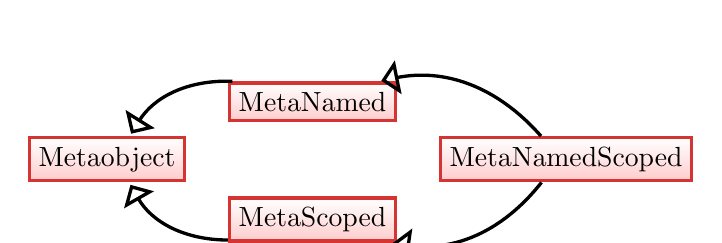
\begin{tikzpicture}
\node [concept] (Metaobject) {Metaobject};
\node [concept] (MetaNamed)[above right=of Metaobject] {MetaNamed}
	edge [inheritance, bend right] (Metaobject);
\node [concept] (MetaScoped)[below right=of Metaobject] {MetaScoped}
	edge [inheritance, bend left] (Metaobject);
\node [concept] (MetaNamedScoped)[below right=of MetaNamed, above right=of MetaScoped] {MetaNamedScoped}
	edge [inheritance, bend right] (MetaNamed)
	edge [inheritance, bend left] (MetaScoped);
\end{tikzpicture}

Models of \meta{NamedScoped} combine the requirements of \meta{Named} and \meta{Scoped}.

%\subsection{MetaScope}
\label{concept-MetaScope}

\meta{Scope} is a \meta{NamedScoped} reflecting program constructs defined inside
of a named or anonymous scope (like the global scope, a namespace, a class, etc.)

In addition to the requirements inherited from \meta{NamedScoped}, the following is required:

The \verb@is_scope@ template class specialization for a \meta{Scope} should
inherit from \verb@true_type@:

\begin{minted}{cpp}
template <>
struct is_scope<MetaScope>
 : true_type
{ };
\end{minted}

\subsubsection{\texttt{members}}

A template class \verb@members@ should be defined and should inherit from a
\concept{MetaobjectSequence} containing \meta{NamedScoped} metaobjects reflecting
the members of the base-level scope reflected by this \meta{Scope}.

Furthermore the boolean \verb@All@ parameter (defaulting to \verb@false@ if not specified)
should control which scope members are listed in the resulting metaobject sequence.

If \verb@All@ is 
\begin{itemize}
\item \verb@true@, then all members should be listed,
\item \verb@false@, then the following scope member should {\em not} be included:
	\begin{itemize}
	\item private or protected class members,
	\item scope members with identifiers starting with an underscore followed by a
	(uppercase or lowercase) letter,
	\item scope members annotated by a generalized attributes as hidden (for example
	\verb@[[mirror::hidden]]@ or \verb@[[reflection::hidden]]@).
	\end{itemize}
\end{itemize}



\begin{minted}{cpp}
template <typename T, bool All=false>
struct members;

template <>
struct members<MetaScope, true>
 : MetaobjectSequence<MetaNamedScoped> // all members
{ };

template <>
struct members<MetaScope, false>
 : MetaobjectSequence<MetaNamedScoped> // only 'visible' members
{ };
\end{minted}


%\subsection{MetaPositional}
\label{concept-MetaPositional}

\meta{Positional} is a \meta{object}, which is fixed to an ordinal position in some context
usually together with other similar metaobjects, like those reflecting parameters of a function,
or the inheritance of base classes, etc.

In addition to the requirements inherited from \meta{object},
the following must be satisfied:

The \verb@has_position@ template class specialization for a \meta{Positional} should
inherit from \verb@true_type@:

\begin{minted}{cpp}
template <>
struct has_position<MetaPositional>
 : true_type
{ };
\end{minted}

\subsubsection{\texttt{position}}

A template class \verb@position@ should be defined and should
inherit from \verb@integral_constant<size_t, I>@ type where \verb@I@ is
a zero-based position (index) of the reflected base-level language construct,
for example the position of a parameter in a list of function parameters,
or the position of an inheritance clause in the list of base classes.

\begin{minted}{cpp}
template <typename T>
struct position;

template <>
struct position<MetaPositional>
 : integral_constant<size_t, I>
{ };
\end{minted}


%\subsection{MetaClassMember}
\label{concept-MetaClassMember}

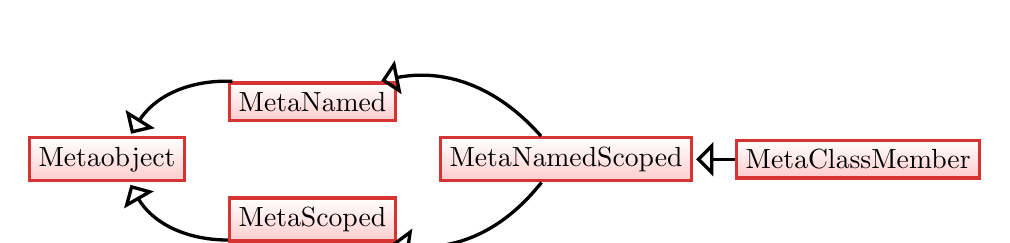
\begin{tikzpicture}
\node [concept] (Metaobject) {Metaobject};
\node [concept] (MetaNamed)[above right=of Metaobject] {MetaNamed}
	edge [inheritance, bend right] (Metaobject);
\node [concept] (MetaScoped)[below right=of Metaobject] {MetaScoped}
	edge [inheritance, bend left] (Metaobject);
\node [concept] (MetaNamedScoped)[below right=of MetaNamed, above right=of MetaScoped] {MetaNamedScoped}
	edge [inheritance, bend right] (MetaNamed)
	edge [inheritance, bend left] (MetaScoped);
\node [concept] (MetaClassMember)[right=of MetaNamedScoped] {MetaClassMember}
	edge [inheritance] (MetaNamedScoped);
\end{tikzpicture}

\meta{Class} is a \meta{Type} and a \meta{Scope} if reflecting a regular class or possibly
also a \meta{Template} if it reflects a class template.

In addition to the requirements inherited from \meta{NamedScoped},
the following is required for \meta{ClassMember}s:

The \verb@is_class_member@ template class specialization for a \meta{ClassMember} should
inherit from \verb@true_type@:

\begin{minted}{cpp}
template <>
struct is_class_member<MetaClassMember>
 : true_type
{ };
\end{minted}

\subsubsection{\texttt{access\_specifier}}

A template class called \verb@access_specifier@ should be defined and should inherit from
a \meta{Specifier} reflecting the \verb@private@, \verb@protected@ or \verb@public@
access specifier:

\begin{minted}{cpp}
template <typename T>
struct access_specifier;

template <>
struct access_specifier<MetaClassMember>
 : MetaSpecifier
{ };
\end{minted}


%\subsection{MetaGlobalScope}
\label{concept-MetaGlobalScope}

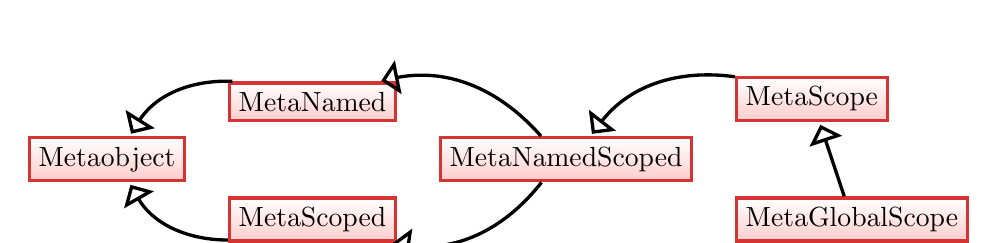
\begin{tikzpicture}
\node [concept] (Metaobject) {Metaobject};
\node [concept] (MetaNamed)[above right=of Metaobject] {MetaNamed}
	edge [inheritance, bend right] (Metaobject);
\node [concept] (MetaScoped)[below right=of Metaobject] {MetaScoped}
	edge [inheritance, bend left] (Metaobject);
\node [concept] (MetaNamedScoped)[below right=of MetaNamed, above right=of MetaScoped] {MetaNamedScoped}
	edge [inheritance, bend right] (MetaNamed)
	edge [inheritance, bend left] (MetaScoped);
\node [concept] (MetaScope)[above right=of MetaNamedScoped] {MetaScope}
	edge [inheritance, bend right] (MetaNamedScoped);
\node [concept] (MetaGlobalScope)[below right=of MetaNamedScoped] {MetaGlobalScope}
	edge [inheritance] (MetaScope);
\end{tikzpicture}

\meta{GlobalScope} is a \meta{Scope} reflecting the global scope.

In addition to the requirements inherited from \meta{Scope}, the following must
be satisfied:

The \verb@metaobject_category@ template class specialization for a \meta{GlobalScope} should
inherit from \verb@global_scope_tag@:

\begin{minted}{cpp}
template <>
struct metaobject_category<MetaNamespace>
 : global_scope_tag
{ };
\end{minted}

The \verb@scope@ template class specialization (required by \meta{Scoped}) for \meta{GlobalScope}
should inherit from the \meta{GlobalScope} itself:

\begin{minted}{cpp}
template <>
struct scope<MetaGlobalScope>
 : MetaGlobalScope
{ };
\end{minted}


%\subsection{MetaNamespace}
\label{concept-MetaNamespace}

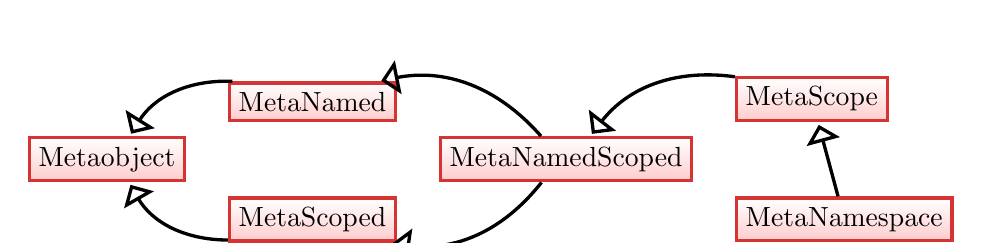
\begin{tikzpicture}
\node [concept] (Metaobject) {Metaobject};
\node [concept] (MetaNamed)[above right=of Metaobject] {MetaNamed}
	edge [inheritance, bend right] (Metaobject);
\node [concept] (MetaScoped)[below right=of Metaobject] {MetaScoped}
	edge [inheritance, bend left] (Metaobject);
\node [concept] (MetaNamedScoped)[below right=of MetaNamed, above right=of MetaScoped] {MetaNamedScoped}
	edge [inheritance, bend right] (MetaNamed)
	edge [inheritance, bend left] (MetaScoped);
\node [concept] (MetaScope)[above right=of MetaNamedScoped] {MetaScope}
	edge [inheritance, bend right] (MetaNamedScoped);
\node [concept] (MetaNamespace)[below right=of MetaNamedScoped] {MetaNamespace}
	edge [inheritance] (MetaScope);
\end{tikzpicture}

\meta{Namespace} is a \meta{Scope} reflecting a namespace.

In addition to the requirements inherited from \meta{Scope}, the following must
be satisfied:

The \verb@metaobject_category@ template class specialization for a \meta{Namespace} should
inherit from \verb@namespace_tag@:

\begin{minted}{cpp}
template <>
struct metaobject_category<MetaNamespace>
 : namespace_tag
{ };
\end{minted}


%\subsection{MetaType}
\label{concept-MetaType}

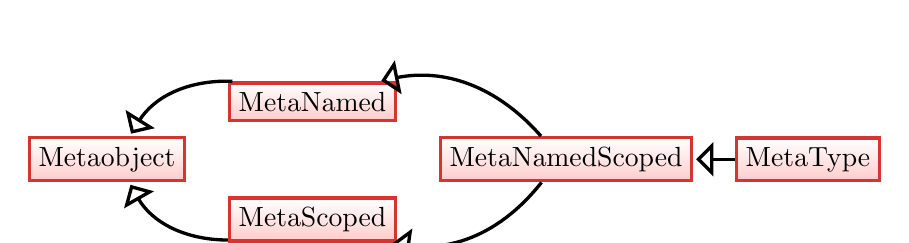
\begin{tikzpicture}
\node [concept] (Metaobject) {Metaobject};
\node [concept] (MetaNamed)[above right=of Metaobject] {MetaNamed}
	edge [inheritance, bend right] (Metaobject);
\node [concept] (MetaScoped)[below right=of Metaobject] {MetaScoped}
	edge [inheritance, bend left] (Metaobject);
\node [concept] (MetaNamedScoped)[below right=of MetaNamed, above right=of MetaScoped] {MetaNamedScoped}
	edge [inheritance, bend right] (MetaNamed)
	edge [inheritance, bend left] (MetaScoped);
\node [concept] (MetaType)[right=of MetaNamedScoped] {MetaType}
	edge [inheritance] (MetaNamedScoped);
\end{tikzpicture}

\meta{Type} is a \meta{NamedScoped} reflecting types.

In addition to the requirements inherited from \meta{NamedScoped}, the following is required:

The \verb@metaobject_category@ template class specialization for a \meta{Type} should
inherit from \verb@type_tag@:

\begin{minted}{cpp}
template <>
struct metaobject_category<MetaType>
 : type_tag
{ };
\end{minted}

\subsubsection{\texttt{original\_type}}

A template class \verb@original_type@ should be defined and should "return"
the original type reflected by this \meta{Type}:

\begin{minted}{cpp}
template <typename T>
struct original_type;

template <>
struct original_type<MetaType>
{
	static_assert(not(is_template<MetaType>::value), "");
	typedef original-type type;
};
\end{minted}

For example, if \verb@__meta_int@ is a metaobject reflecting the \verb@int@ type,
then the specialization of \verb@original_type@ should be following:

\begin{minted}{cpp}
template <>
struct original_type<__meta_int>
{
	typedef int type;
};
\end{minted}

\textbf{Note:} If a concept derived from \meta{Type}, for example a \meta{Class},
is also a \meta{Template} (i.e. is reflecting a template not a concrete type),
then the \verb@original_type@ template should be left undefined.


%\subsection{MetaTypedef}
\label{concept-MetaTypedef}

\meta{Typedef} is a \meta{Type} reflecting \verb@typedef@s.

In addition to the requirements inherited from \meta{Type}, the following is required:

The \verb@category@ template class specialization for a \meta{Typedef} should
inherit from \verb@typedef_tag@:

\begin{minted}{cpp}
template <>
struct category<MetaTypedef>
 : typedef_tag
{ };
\end{minted}

\subsubsection{\texttt{decl\_type}}

A template class called \verb@decl_type@ should be defined and should inherit from the \meta{Type}
reflecting the "source" type of the typedef:

\begin{minted}{cpp}
template <typename T>
struct decl_type;

template <>
struct decl_type<MetaTypedef>
 : MetaType
{ };
\end{minted}

For example if \verb@__meta_std_string@ is a \meta{Typedef} reflecting the \verb@std::string@
typedef and \verb@__meta_std_basic_string_char@ is the \meta{Type} that reflects
the \verb@std::basic_string<char>@ type, and \verb@std::string@ is defined as:

\begin{minted}{cpp}
namespace std {
typedef basic_string<char> string;
}
\end{minted}

then the specialization of \verb@decl_type@ for \verb@__meta_std_string@ should be following:

\begin{minted}{cpp}
template <>
struct decl_type<__meta_std_string>
 : __meta_std_basic_string_char
{ };
\end{minted}

\textbf{Note:} If this feature proves to be too difficult to implement 
at this point\footnote{since some compilers do not keep typedef information},
it can be added later. We, however, think that leaving it out completely would
seriously limit the utility of reflection in certain use cases.

%\subsection{MetaClass}
\label{concept-MetaClass}

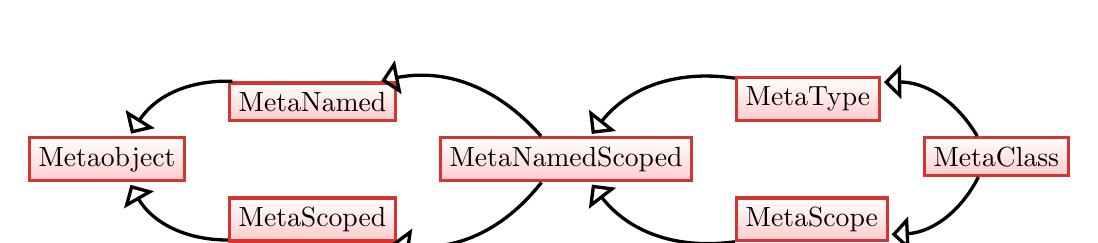
\begin{tikzpicture}
\node [concept] (Metaobject) {Metaobject};
\node [concept] (MetaNamed)[above right=of Metaobject] {MetaNamed}
	edge [inheritance, bend right] (Metaobject);
\node [concept] (MetaScoped)[below right=of Metaobject] {MetaScoped}
	edge [inheritance, bend left] (Metaobject);
\node [concept] (MetaNamedScoped)[below right=of MetaNamed, above right=of MetaScoped] {MetaNamedScoped}
	edge [inheritance, bend right] (MetaNamed)
	edge [inheritance, bend left] (MetaScoped);
\node [concept] (MetaType)[above right=of MetaNamedScoped] {MetaType}
	edge [inheritance, bend right] (MetaNamedScoped);
\node [concept] (MetaScope)[below right=of MetaNamedScoped] {MetaScope}
	edge [inheritance, bend left] (MetaNamedScoped);
\node [concept] (MetaClass)[below right=of MetaType] {MetaClass}
	edge [inheritance, bend right] (MetaType)
	edge [inheritance, bend left] (MetaScope);
\end{tikzpicture}

\meta{Class} is a \meta{Type} and a \meta{Scope} if reflecting a regular class or possibly
also a \meta{Template} if it reflects a class template.

In addition to the requirements inherited from \meta{Type}, \meta{Scope}
and optionally from \meta{Template},
models of \meta{Class} are subject to the following:

The \verb@metaobject_category@ template class specialization for a \meta{Class} should
inherit from \verb@class_tag@:

\begin{minted}{cpp}
template <>
struct metaobject_category<MetaClass>
 : class_tag
{ };
\end{minted}

If a \meta{Class} reflects a class template, then the \verb@is_template@
trait should inherit from \verb@true_type@

\subsubsection{\texttt{elaborated\_type\_specifier}}

A template class called \verb@elaborated_type_specifier@ should be defined and should inherit from
a \meta{Specifier} reflecting the \verb@class@, \verb@struct@ or \verb@union@
specifiers:

\begin{minted}{cpp}
template <typename T>
struct elaborated_type_specifier;

template <>
struct elaborated_type_specifier<MetaClass>
 : MetaSpecifier
{ };
\end{minted}

\subsubsection{\texttt{base\_classes}}

A template class \verb@base_classes@ should be defined and should inherit from
a \concept{MetaobjectSequence} of \meta{Inheritance}s, each one of which reflects the inheritance
of a single base class of the class reflected by the \meta{Class}:

\begin{minted}{cpp}
template <typename T>
struct base_classes;

template <>
struct base_classes<MetaClass>
 : MetaobjectSequence<MetaInheritance>
{ };
\end{minted}


%\subsection{MetaEnum}
\label{concept-MetaEnum}

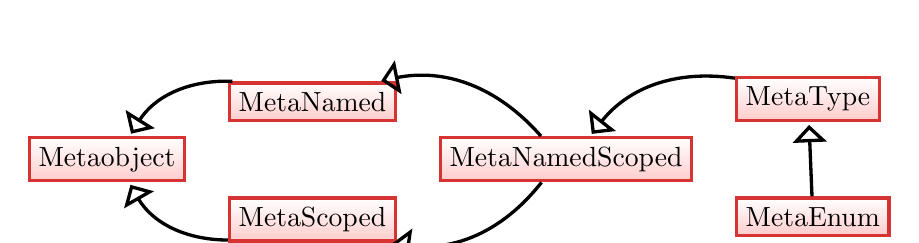
\begin{tikzpicture}
\node [concept] (Metaobject) {Metaobject};
\node [concept] (MetaNamed)[above right=of Metaobject] {MetaNamed}
	edge [inheritance, bend right] (Metaobject);
\node [concept] (MetaScoped)[below right=of Metaobject] {MetaScoped}
	edge [inheritance, bend left] (Metaobject);
\node [concept] (MetaNamedScoped)[below right=of MetaNamed, above right=of MetaScoped] {MetaNamedScoped}
	edge [inheritance, bend right] (MetaNamed)
	edge [inheritance, bend left] (MetaScoped);
\node [concept] (MetaType)[above right=of MetaNamedScoped] {MetaType}
	edge [inheritance, bend right] (MetaNamedScoped);
\node [concept] (MetaEnum)[below right=of MetaNamedScoped] {MetaEnum}
	edge [inheritance] (MetaType);
\end{tikzpicture}

\meta{Enum} is a \meta{Type} reflecting an enumeration type.

In addition to the requirements inherited from \meta{Type}, \meta{Enum} requires
also the following:

The \verb@metaobject_category@ template class specialization for a \meta{Enum} should
inherit from \verb@enum_tag@:

\begin{minted}{cpp}
template <>
struct metaobject_category<MetaEnum>
 : enum_tag
{ };
\end{minted}

\subsubsection{\texttt{base\_type}}

A template class \verb@base_type@ should be defined and should inherit from
a \meta{Type} reflecting the underlying type of the enumeration:

\begin{minted}{cpp}
template <typename T>
struct base_type;

template <>
struct base_type<MetaEnum>
 : MetaType
{ };
\end{minted}

\subsubsection{\texttt{elaborated\_type\_specifier}}

A template class called \verb@elaborated_type_specifier@ should be defined and should inherit from
a \meta{Specifier} reflecting the \verb@enum@ specifier:

\begin{minted}{cpp}
template <typename T>
struct elaborated_type_specifier;

template <>
struct elaborated_type_specifier<MetaEnum>
 : MetaSpecifier
{ };
\end{minted}

\subsubsection{\texttt{members}}

A template class \verb@members@ should be defined and should inherit from a
\concept{MetaobjectSequence} containing \meta{NamedScoped} \meta{Constant} metaobjects
reflecting all enumerated values of the base-level enum reflected by
this \meta{Enum}. The \verb@scope@ of the enumeration values is however not the
containing \verb@enum@, but the scope of that \verb@enum@.

\begin{minted}{cpp}
template <typename T>
struct members;

template <>
struct members<MetaEnum>
 : MetaobjectSequence<MetaConstant>
{ };
\end{minted}


%\subsection{MetaEnumClass}
\label{concept-MetaEnumClass}

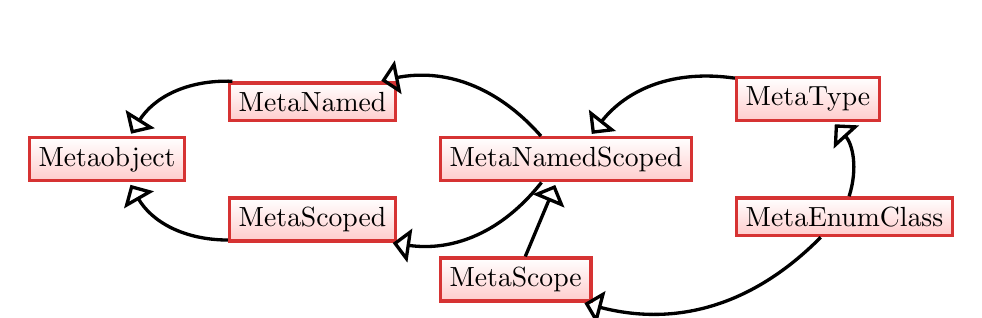
\begin{tikzpicture}
\node [concept] (Metaobject) {Metaobject};
\node [concept] (MetaNamed)[above right=of Metaobject] {MetaNamed}
	edge [inheritance, bend right] (Metaobject);
\node [concept] (MetaScoped)[below right=of Metaobject] {MetaScoped}
	edge [inheritance, bend left] (Metaobject);
\node [concept] (MetaNamedScoped)[below right=of MetaNamed, above right=of MetaScoped] {MetaNamedScoped}
	edge [inheritance, bend right] (MetaNamed)
	edge [inheritance, bend left] (MetaScoped);
\node [concept] (MetaType)[above right=of MetaNamedScoped] {MetaType}
	edge [inheritance, bend right] (MetaNamedScoped);
\node [concept] (MetaScope)[below right=of MetaScoped] {MetaScope}
	edge [inheritance] (MetaNamedScoped);
\node [concept] (MetaEnumClass)[below right=of MetaNamedScoped] {MetaEnumClass}
	edge [inheritance, bend right] (MetaType)
	edge [inheritance, bend left] (MetaScope);
\end{tikzpicture}

\meta{EnumClass} is a \meta{Type} and a \meta{Scope} reflecting a strongly type enumeration.

In addition to the requirements inherited from \meta{Type} and \meta{Scope}, the following must
be satisfied:

The \verb@metaobject_category@ template class specialization for a \meta{EnumClass} should
inherit from \verb@enum_class_tag@:

\begin{minted}{cpp}
template <>
struct metaobject_category<MetaEnumClass>
 : enum_class_tag
{ };
\end{minted}

The \verb@members@ of \meta{EnumClass} are only \meta{NamedScoped} \meta{Constant}s.

\subsubsection{\texttt{base\_type}}

A template class \verb@base_type@ should be defined and should inherit from
a \meta{Type} reflecting the base type of the enumeration:

\begin{minted}{cpp}
template <typename T>
struct base_type;

template <>
struct base_type<MetaEnumClass>
 : MetaType
{ };
\end{minted}

\subsubsection{\texttt{elaborated\_type\_specifier}}

A template class called \verb@elaborated_type_specifier@ should be defined and should inherit from
a \meta{Specifier} reflecting the \verb@enum class@ specifier:

\begin{minted}{cpp}
template <typename T>
struct elaborated_type_specifier;

template <>
struct elaborated_type_specifier<MetaEnumClass>
 : MetaSpecifier
{ };
\end{minted}

%\subsection{MetaOverloadedFunction}
\label{concept-MetaOverloadedFunction}

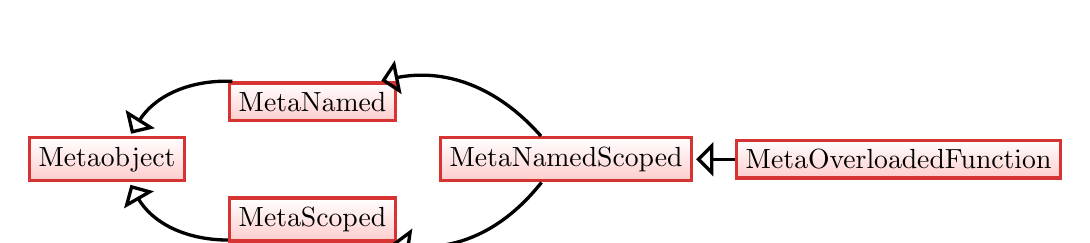
\begin{tikzpicture}
\node [concept] (Metaobject) {Metaobject};
\node [concept] (MetaNamed)[above right=of Metaobject] {MetaNamed}
	edge [inheritance, bend right] (Metaobject);
\node [concept] (MetaScoped)[below right=of Metaobject] {MetaScoped}
	edge [inheritance, bend left] (Metaobject);
\node [concept] (MetaNamedScoped)[below right=of MetaNamed, above right=of MetaScoped] {MetaNamedScoped}
	edge [inheritance, bend right] (MetaNamed)
	edge [inheritance, bend left] (MetaScoped);
\node [concept] (MetaOverloadedFunction)[right=of MetaNamedScoped] {MetaOverloadedFunction}
	edge [inheritance] (MetaNamedScoped);
\end{tikzpicture}


Models of \meta{OverloadedFunction} reflect overloaded functions.
\meta{Function}s (and \meta{Operator}s, \meta{Initializer}s, \meta{Constructor}s, etc.)
are not direct members of scopes (they are not listed in the \concept{MetaobjectSequence}
"returned" by the \verb@members<MetaScope>@ template class).
Instead, all functions, operators and constructors with the same name, (and even those that are not
overloaded in a specific scope) are grouped into a \meta{OverloadedFunction}. Individual overloaded \meta{Function}s
in the group can be obtained through the interface of \meta{OverloadedFunction} (specifically through the
\verb@overloads@ template described below). The same also applies to \meta{Constructor}s and \meta{Operator}s.

The rationale for this is that direct scope members, i.e. metaobjects accessible through the \meta{Scope}'s
\verb@members@ template class should have unique names, which would not be the case if \meta{Function}s
were direct scope members.

The \verb@scope@ of an \meta{OverloadedFunction} is the same as the \verb@scope@
of all \meta{Function}s grouped by that \meta{OverloadedFunction}.

In addition to the requirements inherited from \meta{NamedScoped},
models of \meta{OverloadedFunction} are subject to the following:

The \verb@metaobject_category@ template class specialization for a \meta{OverloadedFunction}
should inherit from \verb@overloaded_function_tag@:

\begin{minted}{cpp}
template <>
struct metaobject_category<MetaOverloadedFunction>
 : overloaded_function_tag
{ };
\end{minted}

\subsubsection{\texttt{overloads}}

A template class called \verb@overloads@ should be defined and should
return a \concept{MetaobjectSequence} of \meta{Function}s, reflecting
the individual overloads:

\begin{minted}{cpp}
template <>
struct overloads<MetaOverloadedFunction>
 : MetaobjectSequence<MetaFunction>
{ };
\end{minted}


%\subsection{MetaFunction}
\label{concept-MetaFunction}

\meta{Function} is a \meta{NamedScoped} which reflects a function or a function template.

In addition to the requirements inherited from \meta{NamedScoped},
models of \meta{Function} are subject to the following:

The \verb@metaobject_category@ template class specialization for a \meta{Function} should
inherit from \verb@function_tag@:

\begin{minted}{cpp}
template <>
struct metaobject_category<MetaFunction>
 : function_tag
{ };
\end{minted}

If a \meta{Function} reflects a function template, then the \verb@is_template@
trait should inherit from \verb@true_type@

\subsubsection{\texttt{linkage\_specifier}}

A template class \verb@linkage_specifier@ should be defined and should inherit from
a \meta{Specifier} reflecting the linkage specifier of the function reflected by
the \meta{Function}:

\begin{minted}{cpp}
template <typename T>
struct linkage_specifier;

template <>
struct linkage_specifier<MetaFunction>
 : MetaSpecifier
{ };
\end{minted}

\subsubsection{\texttt{constexpr\_specifier}}

A template class \verb@constexpr_specifier@ should be defined and should inherit from
a \meta{Specifier} reflecting the constexpr specifier of the reflected function:

\begin{minted}{cpp}
template <typename T>
struct constexpr_specifier;

template <>
struct constexpr_specifier<MetaFunction>
 : MetaSpecifier
{ };
\end{minted}

In case the reflected function does not have the \verb@constexpr@ specifier,
then the result should be a \meta{Specifier} reflecting the "none" specifier.

\subsubsection{\texttt{result\_type}}

A template class \verb@result_type@ should be defined and should inherit from
a \meta{Type} reflecting the return value type of the reflected function:

\begin{minted}{cpp}
template <typename T>
struct result_type;

template <>
struct result_type<MetaFunction>
 : MetaType
{ };
\end{minted}

\subsubsection{\texttt{parameters}}

A template class \verb@parameters@ should be defined and should inherit from
a \concept{MetaobjectSequence} or \meta{Parameter}s reflecting the individual parameters
of the function:

\begin{minted}{cpp}
template <typename T>
struct parameters;

template <>
struct parameters<MetaFunction>
 : MetaobjectSequence<MetaParameter>
{ };
\end{minted}

\subsubsection{\texttt{noexcept\_specifier}}

A template class \verb@noexcept_specifier@ should be defined and should inherit from
a \meta{Specifier} reflecting the noexcept specifier of the reflected function:

\begin{minted}{cpp}
template <typename T>
struct noexcept_specifier;

template <>
struct noexcept_specifier<MetaFunction>
 : MetaSpecifier
{ };
\end{minted}

In case the reflected function does not have the \verb@noexcept@ specifier,
then the result should be a \meta{Specifier} reflecting the "none" specifier.

\subsubsection{\texttt{exceptions}}

A template class \verb@exceptions@ should be defined and should inherit from
a \concept{MetaobjectSequence} of \meta{Type}s reflecting the individual exception types
that the reflected function is allowed to throw:

\begin{minted}{cpp}
template <typename T>
struct exceptions;

template <>
struct exceptions<MetaFunction>
 : MetaobjectSequence<MetaType>
{ };
\end{minted}

\subsubsection{\texttt{const\_specifier}}

In case a \meta{Function} is also a \meta{ClassMember},
a template class \verb@const_specifier@ should be defined and should inherit from
a \meta{Specifier} reflecting the \verb@const@ specifier of the reflected member function:

\begin{minted}{cpp}
template <typename T>
struct const_specifier;

template <>
struct const_specifier<MetaFunction>
 : MetaSpecifier
{
	static_assert(is_class_member<MetaFunction>::value, "");
};
\end{minted}

In case the reflected member function does not have the \verb@const@ specifier,
then the result should be a \meta{Specifier} reflecting the "none" specifier.

\subsubsection{\texttt{virtual\_specifier}}

In case a \meta{Function} is also a \meta{ClassMember},
a template class \verb@virtual_specifier@ should be defined and should inherit from
a \meta{Specifier} reflecting the \verb@virtual@ specifier of the reflected member function:

\begin{minted}{cpp}
template <typename T>
struct virtual_specifier;

template <>
struct virtual_specifier<MetaFunction>
 : MetaSpecifier
{
	static_assert(is_class_member<MetaFunction>::value, "");
};
\end{minted}

In case the reflected member function does not have the \verb@virtual@ specifier,
then the result should be a \meta{Specifier} reflecting the "none" specifier.

\subsubsection{\texttt{is\_pure}}

In case a \meta{Function} is also a \meta{ClassMember},
a template class \verb@is_pure@ should be defined and should inherit from
\verb@true_type@ if the reflected function is pure virtual or from \verb@false_type@
otherwise:

\begin{minted}{cpp}
template <typename T>
struct is_pure;

struct is_pure<MetaFunction>
 : std::integral_constant<bool, B>
{
	static_assert(is_class_member<MetaFunction>::value, "");
};
\end{minted}

\subsubsection{\texttt{pointer}}

If the \meta{Function} reflects a namespace-level function, then
a template class \verb@pointer@ should be defined as follows:

\begin{minted}{cpp}
template <typename T>
struct pointer;

template <>
struct pointer<MetaFunction>
{
	typedef _rv_t (*type)(_param_t...);

	static type get(void);
};
\end{minted}

The \verb@get@ static member function should return a pointer to the function
reflected by the \meta{Function}.

If the \meta{Function} is also a \meta{ClassMember}, then the definition of the
\verb@pointer@ template class should be following:

\begin{minted}{cpp}
template <>
struct pointer<MetaFunction>
{
	typedef _rv_t (_cls_t::*type)(_param_t...);

	static type get(void);
};
\end{minted}


%\subsection{MetaInitializer}
\label{concept-MetaInitializer}

\meta{Initializer} reflects an initializer (constructor) of a native type.

In addition to the requirements inherited from \meta{Function},
models of \meta{Initializer} must conform to the following:

The \verb@metaobject_category@ template class specialization for a \meta{Initializer} should
inherit from \verb@constructor_tag@:

\begin{minted}{cpp}
template <>
struct metaobject_category<MetaInitializer>
 : constructor_tag
{ };
\end{minted}

The specialization of the \verb@result_type@ template class for a \meta{Initializer} should
inherit from a \meta{Type} reflecting the initialized type:

\begin{minted}{cpp}
template <>
struct result_type<MetaInitializer>
 : MetaType
{ };
\end{minted}


%\subsection{MetaConstructor}
\label{concept-MetaConstructor}

\meta{Constructor} reflects a constructor of an elaborated type.

In addition to the requirements inherited from \meta{Function} and \meta{ClassMember},
the following is required for \meta{Constructor}s:

The \verb@metaobject_category@ template class specialization for a \meta{Constructor} should
inherit from \verb@constructor_tag@:

\begin{minted}{cpp}
template <>
struct metaobject_category<MetaConstructor>
 : constructor_tag
{ };
\end{minted}

The specialization of the \verb@result_type@ template class for a \meta{Constructor} should
inherit from a \meta{Class} reflecting the constructed type.

\begin{minted}{cpp}
template <>
struct result_type<MetaConstructor>
 : MetaClass
{ };
\end{minted}

The specialization of the \verb@scope@ template class for a \meta{Constructor} should
inherit from a \meta{Class} reflecting the constructed type.

\begin{minted}{cpp}
template <>
struct scope<MetaConstructor>
 : MetaClass
{ };
\end{minted}


%\subsection{MetaOperator}
\label{concept-MetaOperator}


\meta{Operator} is a \meta{Function} which reflects an operator.

In addition to the requirements inherited from \meta{Function},
models of \meta{Operator} must conform to the following:

The \verb@category@ template class specialization for a \meta{Operator} should
inherit from \verb@operator_tag@:

\begin{minted}{cpp}
template <>
struct category<MetaOperator>
 : operator_tag
{ };
\end{minted}


%\subsection{MetaTemplate}
\label{concept-MetaTemplate}

\meta{Template} is a \meta{NamedScoped} and either a \meta{Class} or a \meta{Function}.

\textbf{Note:} The \meta{Template} concept slightly modifies the requirements
of the \meta{Class} and \meta{Function} concepts.

In addition to the requirements inherited from \meta{NamedScoped},
models of \meta{Template} must conform to the following:

The \verb@is_template@ template class specialization for a \meta{Template} should
inherit from \verb@true_type@:

\begin{minted}{cpp}
template <>
struct is_template<MetaTemplate>
 : true_type
{ };
\end{minted}

\subsubsection{\texttt{template\_parameters}}

A template class called \verb@template_parameters@ should be defined and should
inherit from a \concept{MetaobjectSequence} of \meta{TemplateParameter}s,
reflecting the individual type or constant template parameters:

\begin{minted}{cpp}
template <typename T>
struct template_parameters;

template <>
struct template_parameters<MetaTemplate>
 : MetaobjectSequence<MetaTemplateParameter>
{ };
\end{minted}

\subsubsection{\texttt{instantiation}}

A template class \verb@instantiation@ should be defined and should
inherit from a \meta{Instantiation} reflecting a concrete instantiation of
the template reflected by this \meta{Template}:

\begin{minted}{cpp}
template <typename T, typename ... P>
struct instantiation;

template <typename ... P>
struct instantiation<MetaTemplate, P...>
 : MetaInstantiation
{ };
\end{minted}

For example if \verb@__meta_std_pair@ is a \meta{Template} and a \meta{Class} reflecting
the \verb@std::pair@ template and \verb@__meta_std_pair_int_double@ is a \meta{Instantiation}
and a \meta{Class} reflecting the \verb@std::pair<int, double>@ class then:

\begin{minted}{cpp}
static_assert(
	is_base_of<
		__meta_std_pair_int_double,
		instantiation<__meta_std_pair, int, double>
	>() , ""
);
\end{minted}

%\subsection{MetaTemplateParameter}
\label{concept-MetaTemplateParameter}

\meta{TemplateParameter} is a \meta{NamedScoped}, \meta{Positional}
and either a \meta{Type} and \meta{Alias} or a \meta{Constant}.

In addition to the requirements inherited from \meta{NamedScoped},
models of \meta{TemplateParameter} must conform to the following:

The \verb@is_template@ template class specialization for a \meta{TemplateParameter} should
inherit from \verb@true_type@:

\begin{minted}{cpp}
template <>
struct is_template<MetaTemplateParameter>
 : true_type
{ };
\end{minted}

The \verb@full_name@ inherited from \meta{Named} should return the same \concept{StringConstant}
as \verb@base_name@ for models of \meta{TemplateParameter}, i.e. the plain template parameter
name without any qualifications.

\subsubsection{\texttt{is\_pack}}

A template class called \verb@is_pack@ should be defined and should
inherit from \verb@true_type@ if the template parameter is a pack
parameter or from \verb@false_type@ otherwise.

\begin{minted}{cpp}
template <typename T>
struct is_pack;

template <>
struct is_pack<MetaTemplateParameter>
 : integral_constant<bool, B>
{ };
\end{minted}


%\subsection{MetaInstantiation}
\label{concept-MetaInstantiation}

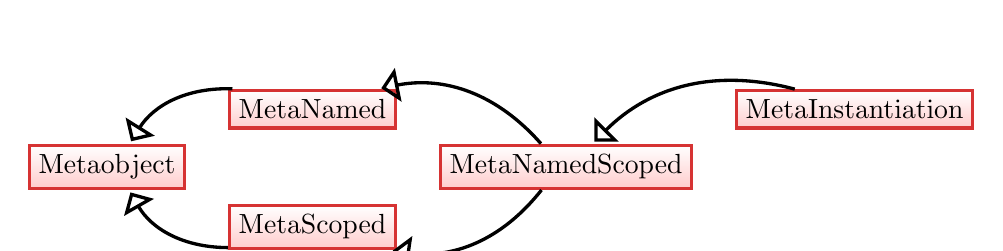
\begin{tikzpicture}
\node [concept] (Metaobject) {Metaobject};
\node [concept] (MetaNamed)[above right=of Metaobject] {MetaNamed}
	edge [inheritance, bend right] (Metaobject);
\node [concept] (MetaScoped)[below right=of Metaobject] {MetaScoped}
	edge [inheritance, bend left] (Metaobject);
\node [concept] (MetaNamedScoped)[below right=of MetaNamed, above right=of MetaScoped] {MetaNamedScoped}
	edge [inheritance, bend right] (MetaNamed)
	edge [inheritance, bend left] (MetaScoped);
\node [concept] (MetaInstantiation)[above right=of MetaNamedScoped] {MetaInstantiation}
	edge [inheritance, bend right] (MetaNamedScoped);
\end{tikzpicture}


\meta{Instantiation} is a \meta{NamedScoped} and either a \meta{Class} or a \meta{Function}.

In addition to the requirements inherited from \meta{NamedScoped},
models of \meta{Instantiation} must conform to the following:

The \verb@has_template@ template class specialization for a \meta{Instantiation} should
inherit from \verb@true_type@:

\begin{minted}{cpp}
template <>
struct has_template<MetaInstantiation>
 : true_type
{ };
\end{minted}

\subsubsection{\texttt{template\_arguments}}

A template class called \verb@template_arguments@ should be defined and should
inherit from a \concept{MetaobjectSequence} of \meta{NamedScoped} metaobjects
each of which is either a \meta{Type} or a \meta{Constant} and reflects
the i-th template argument:

\begin{minted}{cpp}
template <typename T>
struct template_arguments;

template <>
struct template_arguments<MetaInstantiation>
 : MetaobjectSequence<MetaNamedScoped>
{ };
\end{minted}

\subsubsection{\texttt{template\_}}

A template class called \verb@template_@ should be defined and should
inherit from a \meta{Template} reflecting the instantiation's template:

\begin{minted}{cpp}
template <typename T>
struct template_;

template <>
struct template_<MetaInstantiation>
 : MetaTemplate
{ };
\end{minted}

For example if \verb@__meta_std_pair@ is a \meta{Template} and a \meta{Class} reflecting
the \verb@std::pair@ template and \verb@__meta_std_pair_int_double@ is a \meta{Instantiation}
and a \meta{Class} reflecting the \verb@std::pair<int, double>@ class then:

\begin{minted}{cpp}
static_assert(
	is_base_of<
		__meta_std_pair,
		template_<__meta_std_pair_int_double>
	>() , ""
);
\end{minted}

%\subsection{MetaInheritance}
\label{concept-MetaInheritance}

\meta{Inheritance} is a \meta{Scoped} and \meta{Positional} reflecting class inheritance.

In addition to the requirements inherited from \meta{Scoped} and \meta{Positional},
types conforming to this concept must satisfy the following:

The \verb@category@ template should return \verb@inheritance_tag@ for models
of \meta{Inheritance}:

\begin{minted}{cpp}
template <>
struct category<MetaInheritance>
 : inheritance_tag
{ };
\end{minted}

The \verb@scope@ member function should inherit from a \meta{Class} reflecting
the derived class in the inheritance:

\begin{minted}{cpp}
template <>
struct scope<MetaInheritance>
 : MetaClass
{ };
\end{minted}

\subsubsection{\texttt{access\_specifier}}

A template struct \verb@access_specifier@ should be defined and should inherit from
a \meta{Specifier} reflecting one of the \verb@private@, \verb@protected@ and
\verb@public@ access specifiers.

\begin{minted}{cpp}
template <typename T>
struct access_specifier;

template <>
struct access_specifier<MetaInheritance>
 : MetaSpecifier
{ };
\end{minted}

\subsubsection{\texttt{inheritance\_specifier}}

A template struct \verb@inheritance_specifier@ should be defined and should inherit from
a \meta{Specifier} reflecting one of the \verb@virtual@ and "none" access specifiers.

\begin{minted}{cpp}
template <typename T>
struct inheritance_specifier;

template <>
struct inheritance_specifier<MetaInheritance>
 : MetaSpecifier
{ };
\end{minted}

\subsubsection{\texttt{base\_class}}

A template struct \verb@base_class@ should be defined and should inherit from
a \meta{Class} reflecting the base class in the inheritance:

\begin{minted}{cpp}
template <typename T>
struct base_class;

template <>
struct base_class<MetaInheritance>
 : MetaClass
{ };
\end{minted}


%\subsection{MetaVariable}
\label{concept-MetaVariable}

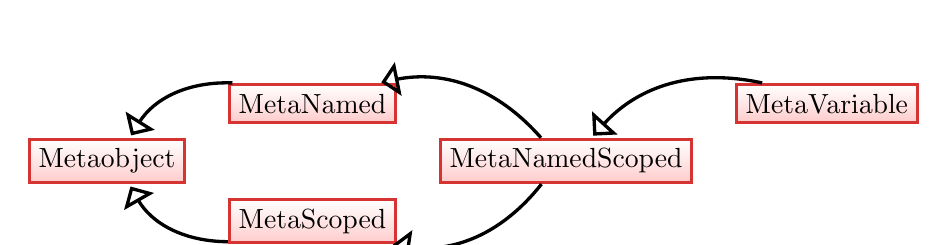
\begin{tikzpicture}
\node [concept] (Metaobject) {Metaobject};
\node [concept] (MetaNamed)[above right=of Metaobject] {MetaNamed}
	edge [inheritance, bend right] (Metaobject);
\node [concept] (MetaScoped)[below right=of Metaobject] {MetaScoped}
	edge [inheritance, bend left] (Metaobject);
\node [concept] (MetaNamedScoped)[below right=of MetaNamed, above right=of MetaScoped] {MetaNamedScoped}
	edge [inheritance, bend right] (MetaNamed)
	edge [inheritance, bend left] (MetaScoped);
\node [concept] (MetaVariable)[above right=of MetaNamedScoped] {MetaVariable}
	edge [inheritance, bend right] (MetaNamedScoped);
\end{tikzpicture}

\meta{Variable} is a \meta{NamedScoped} reflecting a variable.

In addition to the requirements inherited from \meta{NamedScoped}, the following must
be satisfied:

The \verb@metaobject_category@ template class specialization for a \meta{Variable} should
inherit from \verb@variable_tag@:

\begin{minted}{cpp}
template <>
struct metaobject_category<MetaVariable>
 : variable_tag
{ };
\end{minted}

\subsubsection{\texttt{storage\_specifier}}

A template class \verb@storage_specifier@ should be added and should
inherit from a \meta{Specifier} reflecting a storage class specifier:

\begin{minted}{cpp}
template <typename T>
struct storage_specifier;

template <>
struct storage_specifier<MetaVariable>
 : MetaSpecifier
{ };
\end{minted}

\subsubsection{\texttt{type}}

A template class \verb@type@ should be added and should inherit
from a \meta{Type} reflecting the type of the variable:

\begin{minted}{cpp}
template <typename T>
struct type;

template <>
struct type<MetaVariable>
 : MetaType
{ };
\end{minted}

\subsubsection{\texttt{pointer}}

If the reflected variable is a namespace-level variable, then a template
class \verb@pointer@ should be implemented as follows:

\begin{minted}{cpp}
template <typename T>
struct pointer;

template <>
struct pointer<MetaVariable>
{
	typedef typename original_type<type<MetaVariable>>::type* type;

	static type get(void);
};
\end{minted}

The static member function \verb@get@ should return the address of the reflected variable.

If the reflected variable is a class member variable (i.e. if the \meta{Variable}
is also a \meta{ClassMember}), then the \verb@pointer@ template class should be
defined as follows:

\begin{minted}{cpp}

template <>
struct pointer<MetaVariable>
{
	typedef typename original_type<type<MetaVariable>>::type
		_mv_t;
	typedef typename original_type<type<scope<MetaVariable>>>::type
		_cls_t;

	typedef _mv_t _cls_t::* type;

	static type get(void);
};

\end{minted}

The static member function \verb@get@ should return a data member pointer to
the reflected member variable. The \verb@_mv_t@ and \verb@_cls_t@ typedefs
are implementation details and are not a part of this specification.

%\subsection{MetaParameter}
\label{concept-MetaParameter}

\meta{Parameter} is a \meta{Named}, \meta{Scoped} and \meta{Positional},
reflecting a function parameter or a parameter pack.

In addition to the requirements inherited from \meta{Named} and \meta{Scoped},
the following must be satisfied:

The \verb@metaobject_category@ template class specialization for a \meta{Parameter} should
inherit from \verb@parameter_tag@:

\begin{minted}{cpp}
template <>
struct metaobject_category<MetaParameter>
 : parameter_tag
{ };
\end{minted}

The \verb@scope@ of a \meta{Parameter} should be a \meta{Function} reflecting
the function to which the parameter belongs:

\begin{minted}{cpp}
template <>
struct scope<MetaParameter>
 : MetaFunction
{ };
\end{minted}

The \verb@full_name@ inherited from \meta{Named} should return the same \concept{StringConstant}
as \verb@base_name@ for models of \meta{Parameter}, i.e. the plain parameter
name without any qualifications.

\subsubsection{\texttt{is\_pack}}

A template class called \verb@is_pack@ should be defined and should
inherit from \verb@true_type@ if the parameter is a part of an expanded
parameter pack or from \verb@false_type@ otherwise.

\begin{minted}{cpp}
template <typename T>
struct is_pack;

template <>
struct is_pack<MetaParameter>
 : integral_constant<bool, B>
{ };
\end{minted}

When a concrete instantiation of a function template with a parameter pack
is reflected then the individual \meta{Parameter}s reflect the actual parameters
of that instantiation. In such case the \verb@parameters@ template "returns"
a \concept{MetaobjectSequence} of \meta{Parameter}s where some of the \meta{Parameter}
have the same name (the name of the pack template parameter)
and \verb@is_pack@ inherits from \verb@true_type@.

\subsubsection{\texttt{type}}

A template class \verb@type@ should be added and should inherit
from a \meta{Type} reflecting the type of the parameter:

\begin{minted}{cpp}
template <typename T>
struct type;

template <>
struct type<MetaParameter>
 : MetaType
{ };
\end{minted}

\subsubsection{\texttt{pointer}}

A template class \verb@pointer@ should be implemented as follows:

\begin{minted}{cpp}
template <typename T>
struct pointer;

template <>
struct pointer<MetaParameter>
{
	typedef typename original_type<type<MetaParameter>>::type* type;

	static type get(void);
};
\end{minted}

The static member function \verb@get@ should return the address of the reflected parameter
instance if it is invoked (directly or indirectly) inside of the body of the function to which
the reflected parameter belongs to. Otherwise it should return \verb@nullptr@.

In case of recursively called functions, pointers to the arguments of the innermost
invocation should be returned.

%\subsection{MetaConstant}
\label{concept-MetaConstant}

\meta{Constant} is a \meta{object} reflecting a compile-time constant value.

In addition to the requirements inherited from \meta{object}, the following must
be satisfied:

The \verb@category@ template class specialization for a \meta{Constant} should
inherit from \verb@constant_tag@:

\begin{minted}{cpp}
template <>
struct category<MetaConstant>
 : constant_tag
{ };
\end{minted}

\subsubsection{\texttt{type}}

A template class \verb@type@ should be added and should inherit
from a \meta{Type} reflecting the type of the constant value

\begin{minted}{cpp}
template <typename T>
struct type;

template <>
struct type<MetaVariable>
 : MetaType
{ };
\end{minted}

\subsubsection{\texttt{value}}

A template class \verb@value@ should be added and should inherit
from an \verb@integral_constant<T, V>@:

\begin{minted}{cpp}
template <typename T>
struct value;

template <>
struct value<MetaConstant>
 : integral_constant<T, V>
{ };
\end{minted}



\section{Identifier pasting}

As a part of this proposal we suggest to add a new functionality to the core language,
allowing to specify identifiers as compile-time constant C-string literal expression, i.e. expressions
evaluating into values of \verb@constexpr const char [N]@.

This could be implemented either by using a new operator (or recycling an old one),
or maybe by using generalized attributes.
In the examples below the \verb@identifier@ operator is used, but we do not have
any strong preference for the name of this operator.

For example:

\begin{minted}{cpp}

identifier("int") identifier("main")(
	int idenitifier("argc"),
	const identifier("char")* identifier("argv")
)
{
	using namespace identifier("std");
	for(int i=0; i<argc; ++i)
	{
		cout << argv[i] << endl;
	}
	return 0;
}

\end{minted}

would be equivalent to

\begin{minted}{cpp}
int main(int argc, const char* argv)
{
	using namespace std;
	return 0;
}
\end{minted}

The content of the string literal passed as the argument to \verb@identifier@
should be encoded in the source character set and subject to the same restrictions
which are placed on identifiers.

For example:

\begin{minted}{cpp}

class foo
{
	identifier("some-type#") x; // Error

	double identifier("static"); // Error

	float identifier("void"); // Error

	long identifier("<bar>"); // Error

	identifier("std::vector<std::unique_ptr<bar>>") v; // OK
};

\end{minted}

The idea is to replace preprocessor token concatenation with much more
flexible constexpr C++ expressions.
Adding identifier pasting would allow to replace the \verb@named_mem_var@
and \verb@named_typedef@ metafunctions which were in N4111 defined as part of
the interface of \meta{Named} with a much more powerful feature.


\section{Examples}

This section contains multiple examples of usage of the additions proposed above.
The examples assume that the \verb@mirrored@ operator (described above) is used
to obtain the metaobjects and the types, templates, etc. are defined in the
\verb@std::meta@ namespace.

For the sake of brevity

\begin{minted}{cpp}
using namespace std;
\end{minted}

is assumed.

\subsection{Basic traits}

Usage of the \verb@is_metaobject@ trait on non-metaobjects:

\begin{minted}[tabsize=4]{cpp}
static_assert(not(is_metaobject<int>()), "");
static_assert(not(is_metaobject<std::string>()), "");
static_assert(not(is_metaobject<my_class>()), "");
static_assert(not(meta::is_class_member<meta_gs>()), "");
\end{minted}


\subsection{Global scope reflection}

\begin{minted}[tabsize=4]{cpp}
// reflected global scope
typedef mirrored(::) meta_gs;

static_assert(is_metaobject<meta_gs>(), "");

// Is a MetaNamed
static_assert(meta::has_name<meta_gs>(), "");
// Is a MetaScoped
static_assert(meta::has_scope<meta_gs>(), "");
// Is a MetaScope
static_assert(meta::is_scope<meta_gs>(), "");
// Is not a MetaClassMember
static_assert(not(meta::is_class_member<meta_gs>()), "");

// Is a MetaGlobalScope
static_assert(
	is_base_of<
		meta::global_scope_tag,
		meta::category<meta_gs>
	>(), ""
);

// Global scope is its own scope
static_assert(
	is_base_of<
		meta_gs,
		meta::scope<meta_gs>
	>(), ""
);

// Empty base and full name
assert(strlen(meta::base_name<meta_gs>()) == 0);
assert(strcmp(meta::base_name<meta_gs>(), "") == 0);

assert(strlen(meta::full_name<meta_gs>()) == 0);
assert(strcmp(meta::full_name<meta_gs>(), "") == 0);

// the sequence of members
typedef meta::members<meta_gs>::type meta_gs_members;

static_assert(
	meta::size<meta_gs_members>() == 20, // YMMV
	""
);

\end{minted}


\subsection{Namespace reflection}

\begin{minted}[tabsize=4]{cpp}
// reflected namespace std
typedef mirrored(std) meta_std;

static_assert(is_metaobject<meta_std>(), "");

// Is a MetaNamed
static_assert(meta::has_name<meta_std>(), "");
// Is a MetaScoped
static_assert(meta::has_scope<meta_std>(), "");
// Is a MetaScope
static_assert(meta::is_scope<meta_std>(), "");
// Is not a MetaClassMember
static_assert(not(meta::is_class_member<meta_std>()), "");

// Is a MetaNamespace
static_assert(
	is_base_of<
		meta::namespace_tag,
		metaobject_category<meta_std>
	>(), ""
);

// The scope of namespace std is the global scope
static_assert(
	is_base_of<
		meta_gs,
		meta::scope<meta_std>
	>(), ""
);

// The base and full name
assert(strlen(meta::base_name<meta_std>()) == 3);
assert(strcmp(meta::base_name<meta_std>(), "std") == 0);
assert(strlen(meta::full_name<meta_std>()) == 3);
assert(strcmp(meta::full_name<meta_std>(), "std") == 0);
\end{minted}

\subsection{Type reflection}

\begin{minted}[tabsize=4]{cpp}
// reflected type unsigned int
typedef mirrored(unsigned int) meta_uint;

static_assert(is_metaobject<meta_uint>(), "");

// Is a MetaNamed
static_assert(meta::has_name<meta_uint>(), "");
// Is a MetaScoped
static_assert(meta::has_scope<meta_uint>(), "");
// Is not a MetaScope
static_assert(not(meta::is_scope<meta_uint>()), "");
// Is not a MetaClassMember
static_assert(not(meta::is_class_member<meta_uint>()), "");

// Is a MetaType
static_assert(
	is_base_of<
		meta::type_tag,
		meta::category<meta_uint>
	>(), ""
);

// The scope of unsigned int is the global scope
static_assert(
	is_base_of<
		meta_gs,
		meta::scope<meta_uint>
	>(), ""
);

// The original type
static_assert(
	is_same<
		unsigned int,
		meta::original_type<meta_uint>::type
	>(), ""
);

assert(strlen(meta::base_name<meta_uint>()) == 12);
assert(strcmp(meta::base_name<meta_uint>(), "unsigned int") == 0);
assert(strlen(meta::full_name<meta_uint>()) == 12);
assert(strcmp(meta::full_name<meta_uint>(), "unsigned int") == 0);
\end{minted}

\subsection{Typedef reflection}

\begin{minted}[tabsize=4]{cpp}
// reflected typedef std::size_t
typedef mirrored(std::size_t) meta_size_t;

static_assert(is_metaobject<meta_size_t>(), "");

static_assert(meta::has_name<meta_size_t>(), "");
static_assert(meta::has_scope<meta_size_t>(), "");
static_assert(not(meta::is_scope<meta_size_t>()), "");
static_assert(not(meta::is_class_member<meta_size_t>()), "");

// Is a MetaTypedef
static_assert(
	meta::is_alias<meta_size_t>(), ""
);

// The scope of std::size_t is the namespace std
static_assert(
	is_base_of<
		meta_std,
		meta::scope<meta_size_t>
	>(), ""
);

// The original type
static_assert(
	is_same<
		std::size_t,
		meta::original_type<meta_size_t>::type
	>(), ""
);

// the "source" type of the typedef
typedef meta::type<meta_size_t>::type meta_size_t_type;
static_assert(
	is_base_of<
		meta::type_tag,
		meta::category<meta_size_t_type>
	>(), ""
);

// The original type
static_assert(
	is_same<
		std::size_t,
		meta::original_type<meta_size_t_type>::type
	>(), ""
);

assert(strlen(meta::base_name<meta_size_t>()) == 6);
assert(strcmp(meta::base_name<meta_size_t>(), "size_t") == 0);
assert(strlen(meta::full_name<meta_size_t>()) == 11);
assert(strcmp(meta::full_name<meta_size_t>(), "std::size_t") == 0);
// YMMV
assert(strlen(meta::base_name<meta_size_t_type>()) == 12);
assert(strcmp(meta::base_name<meta_size_t_type>(), "unsigned int") == 0);
\end{minted}


\subsection{Class reflection}

\begin{minted}[tabsize=4]{cpp}
struct A
{
	int a;
};

class B
{
private:
	bool b;
public:
	typedef int T;
};

class C
 : public A
 , virtual protected B
{
public:
	static constexpr char c = 'C';

	struct D : A
	{
		static double d;
	} d;
};

union U
{
	long u;
	float v;
};

typedef mirrored(A) meta_A;
typedef mirrored(B) meta_B;
typedef mirrored(C) meta_C;
typedef mirrored(C::D) meta_D;
typedef mirrored(B::T) meta_T;
typedef mirrored(U) meta_U;

// classes are scopes
static_assert(meta::is_scope<meta_A>(), "");
static_assert(meta::is_scope<meta_B>(), "");
static_assert(meta::is_scope<meta_C>(), "");
static_assert(meta::is_scope<meta_D>(), "");
static_assert(meta::is_scope<meta_U>(), "");

// A, B, C, C::D and U are all elaborated types
assert(is_base_of<meta::class_tag, metaobject_category<meta_A>>());
assert(is_base_of<meta::class_tag, metaobject_category<meta_B>>());
assert(is_base_of<meta::class_tag, metaobject_category<meta_C>>());
assert(is_base_of<meta::class_tag, metaobject_category<meta_D>>());
assert(is_base_of<meta::class_tag, metaobject_category<meta_U>>());

static_assert(!meta::is_class_member<meta_A>(), "");
static_assert(!meta::is_class_member<meta_B>(), "");
static_assert(!meta::is_class_member<meta_C>(), "");
static_assert( meta::is_class_member<meta_D>(), "");
static_assert( meta::is_class_member<meta_T>(), "");
static_assert(!meta::is_class_member<meta_U>(), "");

// typenames
assert(strcmp(meta::base_name<meta_A>(), "A") == 0);
assert(strcmp(meta::base_name<meta_B>(), "B") == 0);
assert(strcmp(meta::full_name<meta_D>(), "C::D") == 0);

// reflected elaborated type specifiers for A, B and U
typedef meta::elaborated_type_specifier<meta_A>::type meta_A_ets;
typedef meta::elaborated_type_specifier<meta_B>::type meta_B_ets;
typedef meta::elaborated_type_specifier<meta_U>::type meta_U_ets;

// specifier keywords
assert(strcmp(meta::keyword<meta_A_ets>(), "struct") == 0);
assert(strcmp(meta::keyword<meta_B_ets>(), "class") == 0);
assert(strcmp(meta::keyword<meta_U_ets>(), "union") == 0);

// specifier tags
assert(is_base_of<meta::struct_tag, meta::specifier_category<meta_A_ets>>());
assert(is_base_of< meta::class_tag, meta::specifier_category<meta_B_ets>>());
assert(is_base_of<meta::union_tag, meta::specifier_category<meta_U_ets>>());

// reflected sequences of members of the A,B and C classes
typedef meta::members<meta_A>::type meta_A_members;
typedef meta::members<meta_B>::type meta_B_members;
typedef meta::members<meta_C>::type meta_C_members;

static_assert(meta::size<meta_A_members>() == 1, ""); // A::a
static_assert(meta::size<meta_B_members>() == 2, ""); // B::b,B::T
static_assert(meta::size<meta_C_members>() == 3, ""); // C::c,C::D,C::d

// reflected members of B and C
typedef meta::at<meta_B_members, 0>::type meta_B_b;
typedef meta::at<meta_B_members, 1>::type meta_B_T;
typedef meta::at<meta_C_members, 0>::type meta_C_c;
typedef meta::at<meta_C_members, 1>::type meta_C_D;
typedef meta::at<meta_C_members, 2>::type meta_C_d;

assert(is_base_of<meta::variable_tag, metaobject_category<meta_B_b>>());
assert(is_base_of<meta::typedef_tag, metaobject_category<meta_B_T>>());
assert(is_base_of<meta::class_tag, metaobject_category<meta_C_D>>());

// MetaClassMembers
static_assert( meta::is_class_member<meta_B_b>(), "");
static_assert( meta::is_class_member<meta_B_T>(), "");
static_assert( meta::is_class_member<meta_C_D>(), "");
static_assert( meta::is_class_member<meta_C_d>(), "");

// access specifiers
typedef meta::access_specifier<meta_B_B>::type meta_B_b_access;
typedef meta::access_specifier<meta_C_D>::type meta_C_D_access;

// specifier keywords
assert(strcmp(meta::keyword<meta_B_b_access>(), "private") == 0);
assert(strcmp(meta::keyword<meta_C_D_access>(), "public") == 0);

// sequence of base classes of C
typedef meta::base_classes<meta_C>::type meta_C_bases;

static_assert(meta::size<meta_C_bases>() == 2, ""); // A, B

// MetaInheritances of C->A and C->B
typedef meta::at<meta_C_bases, 0>::type meta_C_base_A;
typedef meta::at<meta_C_bases, 1>::type meta_C_base_B;

// inheritance specifiers
typedef meta::inheritance_specifier<meta_C_base_A>::type meta_C_base_A_it;
typedef meta::inheritance_specifier<meta_C_base_B>::type meta_C_base_B_it;

// access specifiers
typedef meta::access_specifier<meta_C_base_A>::type meta_C_base_A_acc;
typedef meta::access_specifier<meta_C_base_B>::type meta_C_base_B_acc;

// specifier keywords
assert(strcmp(meta::keyword<meta_C_base_A_it>(), "") == 0);
assert(strcmp(meta::keyword<meta_C_base_B_it>(), "virtual") == 0);
assert(strcmp(meta::keyword<meta_C_base_A_acc>(), "public") == 0);
assert(strcmp(meta::keyword<meta_C_base_B_acc>(), "protected") == 0);

// specifier tags
static_assert(
	is_base_of<
		meta::none_tag,
		meta::specifier_category<meta_C_base_A_it>
	>(), ""
);
static_assert(
	is_base_of<
		meta::virtual_tag,
		meta::specifier_category<meta_C_base_B_it>
	>(), ""
);
static_assert(
	is_base_of<
		meta::public_tag,
		meta::specifier_category<meta_C_base_A_acc>
	>(), ""
);

// base classes
static_assert(
	is_base_of<
		meta_A,
		meta::base_class<meta_C_base_A>
	>(), ""
);
static_assert(
	is_base_of<
		meta_B,
		meta::base_class<meta_C_base_B>
	>(), ""
);

\end{minted}


\subsection{Enumeration reflection}

\begin{minted}[tabsize=4]{cpp}
enum E
{
	val_a = 1,
	val_b = 2,
	val_c = 3,
	val_d = 4
};

// reflected enumeration
typedef mirrored(E) meta_E;
// reflected enum values
typedef mirrored(val_a) meta_val_a;
typedef mirrored(val_d) meta_val_d;

// enums are not scopes
static_assert(not(meta::is_scope<meta_E>()), "");
// other traits
static_assert(meta::has_scope<meta_E>(), "");
static_assert(meta::has_name<meta_E>(), "");
static_assert(meta::has_scope<meta_val_a>(), "");
static_assert(meta::has_name<meta_val_a>(), "");

// the categories
assert(is_base_of<meta::enum_tag, metaobject_category<meta_E>>());
assert(is_base_of<meta::constant_tag, metaobject_category<meta_val_a>>());

// names
assert(strcmp(meta::base_name<meta_E>(), "E") == 0);
assert(strcmp(meta::base_name<meta_val_a>(), "val_a") == 0);
assert(strcmp(meta::full_name<meta_val_d>(), "val_d") == 0);

%// reflected elaborated type specifiers for E
%typedef meta::elaborated_type_specifier<meta_E>::type meta_E_ets;

%// specifier keyword
%assert(strcmp(meta::keyword<meta_E_ets>(), "enum") == 0);

%// the members
%typedef meta::members<meta_E>::type meta_E_members;

%assert(meta::size<meta_E_members>() == 4);
%assert(is_base_of<meta_val_a, meta::at<meta_E_members, 0>>());
%assert(is_same<meta_val_d, meta::at<meta_E_members, 3>::type>());

// the scope of the enum values is the same
// as the scope of the enum type
assert(is_same<
	meta::scope<meta_E>::type,
	meta::scope<meta_val_a>::type
>());
assert(is_same<
	meta::scope<meta_E>::type,
	meta::scope<meta::at<meta_E_members, 1>>::type
>());

\end{minted}

\subsection{Strongly-typed enumeration reflection}

\begin{minted}[tabsize=4]{cpp}
enum class E : unsigned short
{
	val_a = 1,
	val_b = 2,
	val_c = 3,
	val_d = 4
};

// reflected enumeration
typedef mirrored(E) meta_E;
// reflected enum values
typedef mirrored(E::val_a) meta_E_val_a;
typedef mirrored(E::val_d) meta_E_val_d;

// enum classes are scopes
static_assert(meta::is_scope<meta_E>(), "");
// other traits
static_assert(meta::has_scope<meta_E>(), "");
static_assert(meta::has_name<meta_E>(), "");
static_assert(meta::has_scope<meta_E_val_a>(), "");
static_assert(meta::has_name<meta_E_val_a>(), "");

// the categories
assert(is_base_of<
	meta::enum_class_tag,
	metaobject_category<meta_E>
>());
assert(is_base_of<
	meta::constant_tag,
	metaobject_category<meta_E_val_a>
>());

// names
assert(strcmp(meta::base_name<meta_E>(), "E") == 0);
assert(strcmp(meta::base_name<meta_E_val_a>(), "val_a") == 0);
assert(strcmp(meta::full_name<meta_E_val_d>(), "E::val_d") == 0);

%// reflected elaborated type specifiers for E
%typedef meta::elaborated_type_specifier<meta_E>::type meta_E_ets;

%// specifier keyword
%assert(strcmp(meta::keyword<meta_E_ets>(), "enum class") == 0);

%// the members
%typedef meta::members<meta_E>::type meta_E_members;

%assert(meta::size<meta_E_members>() == 4);
%assert(is_base_of<meta_E_val_a, meta::at<meta_E_members, 0>>());
%assert(is_same<meta_E_val_d, meta::at<meta_E_members, 3>::type>());

// the scope
assert(is_same<meta_E, meta::scope<meta_E_val_a>::type>());
assert(not(is_same<
	meta::scope<meta_E>::type,
	meta::scope<meta::at<meta_E_members, 1>>::type
>()));
assert(is_same<
	meta::scope<meta_E>::type,
	meta::scope<meta::scope<meta::at<meta_E_members, 1>>>::type
>());

\end{minted}


%TODO



\end{appendices}

\end{document}
